\documentclass[]{article}
\usepackage{lmodern}
\usepackage{amssymb,amsmath}
\usepackage{ifxetex,ifluatex}
\usepackage{fixltx2e} % provides \textsubscript
\ifnum 0\ifxetex 1\fi\ifluatex 1\fi=0 % if pdftex
  \usepackage[T1]{fontenc}
  \usepackage[utf8]{inputenc}
\else % if luatex or xelatex
  \ifxetex
    \usepackage{mathspec}
  \else
    \usepackage{fontspec}
  \fi
  \defaultfontfeatures{Ligatures=TeX,Scale=MatchLowercase}
\fi
% use upquote if available, for straight quotes in verbatim environments
\IfFileExists{upquote.sty}{\usepackage{upquote}}{}
% use microtype if available
\IfFileExists{microtype.sty}{%
\usepackage{microtype}
\UseMicrotypeSet[protrusion]{basicmath} % disable protrusion for tt fonts
}{}
\usepackage[unicode=true]{hyperref}
\hypersetup{
            pdftitle={Requirements Analysis and Specification Document - v1.1},
            pdfauthor={Gianpaolo Branca; Luca Butera; Andrea Cini},
            pdfborder={0 0 0},
            breaklinks=true}
\urlstyle{same}  % don't use monospace font for urls
\usepackage{longtable,booktabs}
% Fix footnotes in tables (requires footnote package)
\IfFileExists{footnote.sty}{\usepackage{footnote}\makesavenoteenv{long table}}{}
\usepackage{graphicx,grffile}
\makeatletter
\def\maxwidth{\ifdim\Gin@nat@width>\linewidth\linewidth\else\Gin@nat@width\fi}
\def\maxheight{\ifdim\Gin@nat@height>\textheight\textheight\else\Gin@nat@height\fi}
\makeatother
% Scale images if necessary, so that they will not overflow the page
% margins by default, and it is still possible to overwrite the defaults
% using explicit options in \includegraphics[width, height, ...]{}
\setkeys{Gin}{width=\maxwidth,height=\maxheight,keepaspectratio}
\IfFileExists{parskip.sty}{%
\usepackage{parskip}
}{% else
\setlength{\parindent}{0pt}
\setlength{\parskip}{6pt plus 2pt minus 1pt}
}
\setlength{\emergencystretch}{3em}  % prevent overfull lines
\providecommand{\tightlist}{%
  \setlength{\itemsep}{0pt}\setlength{\parskip}{0pt}}
\setcounter{secnumdepth}{0}
% Redefines (sub)paragraphs to behave more like sections
\ifx\paragraph\undefined\else
\let\oldparagraph\paragraph
\renewcommand{\paragraph}[1]{\oldparagraph{#1}\mbox{}}
\fi
\ifx\subparagraph\undefined\else
\let\oldsubparagraph\subparagraph
\renewcommand{\subparagraph}[1]{\oldsubparagraph{#1}\mbox{}}
\fi

% set default figure placement to htbp
\makeatletter
\def\fps@figure{htbp}
\makeatother

\usepackage[dvipsnames]{xcolor}
\usepackage{listings}
\usepackage{alloy}

\title{\textbf{Requirements Analysis and Specification Document - v1.1}}
\author{Gianpaolo Branca \and Luca Butera \and Andrea Cini \newline}
\date{
\includegraphics{polimi.png}\newpage}

\begin{document}
\maketitle

{
\setcounter{tocdepth}{3}
\tableofcontents
}
\newpage

\subsection{History of changes}\label{history-of-changes}

\begin{longtable}[]{@{}ll@{}}
\toprule
\begin{minipage}[b]{0.11\columnwidth}\raggedright\strut
Version\strut
\end{minipage} & \begin{minipage}[b]{0.83\columnwidth}\raggedright\strut
Changes\strut
\end{minipage}\tabularnewline
\midrule
\endhead
\begin{minipage}[t]{0.11\columnwidth}\raggedright\strut
1.0\strut
\end{minipage} & \begin{minipage}[t]{0.83\columnwidth}\raggedright\strut
Initial release\strut
\end{minipage}\tabularnewline
\begin{minipage}[t]{0.11\columnwidth}\raggedright\strut
1.1\strut
\end{minipage} & \begin{minipage}[t]{0.83\columnwidth}\raggedright\strut
Add specification about the interaction of the system with the
passengers of a ride\strut
\end{minipage}\tabularnewline
\bottomrule
\end{longtable}

\newpage

\subsection{1 Introduction}\label{introduction}

\subsubsection{1.1 Description of the given
problem}\label{description-of-the-given-problem}

We need to develop a system to support an electric car-sharing service,
which have to be accessible for the users via a mobile application and
provide our customers with a robust software infrastructure to manage
their service.

\subsubsection{1.2 Current company
situation}\label{current-company-situation}

The company which wants to provide the car-sharing service is already in
the public transport business, therefore they have already a network of
maintenance operators in the city area that will also autonomously take
care of the recharging stations. They also have an information system
which provides channels for costumer-care, so that we will not need to
provide it in the context of our system. The company also has an
efficient internal communication system to coordinate their staff, it
will be used in our system to be through the provided APIs.

\subsection{2 Goals}\label{goals}

The system must:

\begin{itemize}
\tightlist
\item
  {[}G0{]} Make the user able to access to the system.
\item
  {[}G1{]} Allow the clients to find an available car within a selected
  radius around his or a specified location.
\item
  {[}G2{]} Allow the clients to book a car and pick it up.
\item
  {[}G3{]} Monitor the usage of the car and charge the client with the
  right fare.
\item
  {[}G4{]} Incentivize a correct usage of the service to allow as many
  as possible users to use the same car without the need of the service
  of an operator.
\item
  {[}G5{]} Ensure a correct distribution of cars in the recharging
  stations according to the available plugs.
\item
  {[}G6{]} Allow operators to manage and monitor the state of all the
  cars and notify them when maintenance is needed on a specific vehicle.
\item
  {[}G7{]} Allow management system to set up and modify parameters of
  the system.
\item
  {[}G8{]} Provide a real time, interactive, pleasant and transparent
  user experience.
\end{itemize}

\subsection{3 Boundaries of the system}\label{boundaries-of-the-system}

\begin{itemize}
\tightlist
\item
  The system to fulfill the goals that we have identified will use the
  Google Maps service to locate cars, users, operators and recharging
  stations and to provide the clients with navigation information.
\item
  The system will rely on PayPal as a payment system as it is very
  reliable and a lot of users will appreciate its use.
\item
  The system will provide operators of the company with the information
  needed for the maintenance of the vehicle but won't involved in the
  coordination of the maintenance team.
\item
  The system will not be able to check if the user behaves against the
  low, for example the system must ensure that a car is parked in a safe
  area but won't be able to check if the car is correctly parked
  according to the law, anyway all the data concerning car usage are
  collected and therefore it is possible to get to the physical person
  who committed the illicit.
\item
  After the check in the system will not monitor the effective presence
  of other passengers other than the driver. That is done because the
  system would end up being more complicated with a deeper integration
  with the car sensors, and also because this behaviour is tolerated
  (e.g a driver can bring two passengers home, than go ahead and still
  get a discount)
\end{itemize}

\subsection{4 Domain properties and
assumptions}\label{domain-properties-and-assumptions}

\begin{itemize}
\tightlist
\item
  {[}D1{]} The GPS service is always available and provides always the
  right position.
\item
  {[}D2{]} The system cannot prevent theft.
\item
  {[}D3{]} Operators are properly trained by the company to use the
  system and correctly mark cars under maintenance as unavailable.
\item
  {[}D4{]} The plugs availability is correctly communicated to the
  system by the recharging station.
\item
  {[}D5{]} User's mobile phones are equipped with a GPS system and a
  camera and they are always working properly.
\item
  {[}D6{]} The measure of the percentage of battery charge left and the
  estimation of the Km/\% of charge ratio are correct.
\item
  {[}D7{]} The internet connection of the cars is always working.
\item
  {[}D8{]} The user has accepted the terms of use of the application.
\item
  {[}D9{]} Every car is equipped with a display.
\end{itemize}

\subsection{5 Glossary}\label{glossary}

\begin{enumerate}
\def\labelenumi{\arabic{enumi}.}
\tightlist
\item
  Valid credential: Name, surname, birth date, driving license, PayPal
  account, valid e-mail address.
\item
  Current car details: Remaining battery, License plate number, an
  estimation of the remaining autonomy expressed in kilometers
  (calculated at average speed of 50 km/h in city traffic), the name and
  an picture of the car model.
\item
  Money saving option: An option that, if it has been activated, will
  provide the user with the information to find a suitable recharging
  station according to his the destination, the availability of plugs
  and uniform distribution of cars among the stations.
\item
  Safe area: area flagged by the management system as suitable for
  leaving the car and ending the ride.
\item
  Operator: in this document we refer as operator to the employees in
  charge of monitoring the state of the car from dedicated terminals of
  the company.
\item
  On screen notification: is a notification which is displayed on the
  screen located inside the vehicle.
\item
  Plugged: a car is considered plugged when a sensor detects that the
  specific car has been connected to the recharging system.
\item
  Update notification: is a notification sent by e-mail to the users
  which contains every detail of the update and eventually the new terms
  and conditions document.
\item
  Fee: a user can be charged with a fee for an improper use of the
  system, the value of the fee can be customized by the management
  system.
\item
  Busy: a car is marked as busy when ridden by a user or left parked but
  kept booked.
\item
  Ban: a banned user can not book car until his debt has not been
  satisfied.
\item
  Push notification: a notification that pops up in real time on the
  user's mobile phone or in the operator terminal.
\end{enumerate}

\subsection{6 Text assumptions}\label{text-assumptions}

\begin{enumerate}
\def\labelenumi{\arabic{enumi}.}
\tightlist
\item
  Discounts and penalties will be applied only in the case of a ride not
  shorter than 2km, so that the system will not punish users for not
  using poorly charged cars for short rides and will not encourage users
  to use fully charged cars less to get the discount.
\item
  Discounts and penalties percentage values can be customized by the
  management system.
\end{enumerate}

\subsection{7 Actors identifying}\label{actors-identifying}

We have two main actors:

Client: is a person who has dowloaded our application and is registered
to the service.

Operator: is an employee who has access to an interface that allows him
to monitor the state of cars and eventually send assistance.

There are also secondary actors (such as third party service providers).

\subsection{8 Requirements}\label{requirements}

\subsubsection{8.1 Functional
Requirements}\label{functional-requirements}

In the following section we are going to identify the requirements that
our system will have to fulfill to reach the goals.

\begin{itemize}
\item
  {[}G0{]} Make the user able to access to the system.

  \begin{itemize}
  \tightlist
  \item
    {[}R0.1{]} A user must sign up with valid credential.
  \item
    {[}R0.2{]} The system must generate a password for the user and send
    it to him through e-mail.
  \item
    {[}R0.3{]} A user must be able to visualize and modify all his
    personal informations.
  \end{itemize}
\item
  {[}G1{]} Allow the clients to find an available car within a selected
  radius around his or a specified location.

  \begin{itemize}
  \tightlist
  \item
    {[}R1.1{]} The system must be able to retrieve the location of the
    user.
  \item
    {[}R1.2{]} The user must be able to scroll the map of the city to
    find a car or specify the radius (in km) around a selected location
    for the car research.
  \item
    {[}R1.3{]} Upon the selection of a car the system must show an
    informative screen with current car details.
  \end{itemize}
\item
  {[}G2{]} Allow the clients to book a car and pick it up.

  \begin{itemize}
  \tightlist
  \item
    {[}R2.1{]} A client must be able to choose one of the available cars
    and book it.
  \item
    {[}R2.2{]} Once a car has been booked no others reservation can be
    performed by the same client until the first one is pending.
  \item
    {[}R2.3{]} After the reservation has been confirmed to the client,
    he has a maximum of 1 hour to reach the car, unlock it and start the
    engine. If the timeout expires the reservation is cancelled and a
    fee is applied.
  \item
    {[}R2.4{]} The user is able to unlock a booked car trough the app at
    any time after the reservation, however he has a maximum of 15
    minutes to turn it on after the unlocking. If this timeout expires,
    the reservation is cancelled the fee is applied.
  \item
    {[}R2.5{]} The user in order and start the car has to check-in
    scanning a QR code in the car display and then press the physical
    start button.
  \end{itemize}
\item
  {[}G3{]} Monitor the usage of the car and charge the client with the
  right fare.

  \begin{itemize}
  \tightlist
  \item
    {[}R3.1{]} As soon as the engine starts the system must start
    charging the user with a fixed amount for minute and show the
    current price of the ride in the display of the car.
  \item
    {[}R3.2{]} When a car is parked in a safe area and the engine is
    turned off, the system will ask the user through the car display if
    he wants to keep the car busy for at maximum 2h, if the user selects
    `NO' or does nothing and leaves the car, the ride is considered as
    ended. If the user selects `YES' the car is marked as busy.
  \item
    {[}R3.3{]} An user can leave the car he's using and keep it busy
    with a time limit of 2 hours. During this time, since the battery is
    not being used, the management may configure a different fare. When
    the timeout expires if the car hasn't been picked up yet the client
    will be charged with the price of the ride up to that point.
  \item
    {[}R3.4{]} A car parked in a place not marked as safe will be
    considered as busy, but if the client breaks the 2 hours timeout he
    will get a fine for improper use of the service (plus the regular
    price for the ride). The situation will be notified to the operators
    that will be able to choose if the car needs to be moved or not.
  \item
    {[}R3.5{]} If the user drives outside the boundaries of the area of
    the service, the system must detect it, notify it to the user a and
    apply an additional time fare as a penalty. After 30 minutes an
    operator will be notified of the situation.
  \item
    {[}R3.6{]} If the signal of a car is lost for more than 10 minutes,
    an operator will be notified with the last known position.
  \item
    {[}R3.7{]} 5 minutes after the end of the ride the user is charged
    with the right amount and a push notification will be delivered on
    the user's mobile phone. The five minutes delay is necessary to give
    the client the possibility to eventually plug the car and get the
    corresponding discount.
  \item
    {[}R3.8{]} If a user is unable to pay for a ride he will be banned
    from the system until the pending payment will be satisfied.
  \end{itemize}
\item
  {[}G4{]} Incentivize a correct usage of the service to allow as many
  as possible users to use the same car without the need of the service
  of an operator.(Note that discounts and penalties will not be applied
  to short rides, further details in Text Assumption n.1)

  \begin{itemize}
  \tightlist
  \item
    {[}R4.1{]} The system will show in the car display a QR code that
    must be scanned by the user, using the application, to check in. If
    2 or more users check in, in addition to the driver, a discount will
    be applied to the ride.
  \item
    {[}R4.2{]} The system will apply a discount in the case that a car
    is left with more the 50\% of the battery capacity available.
  \item
    {[}R4.3{]} The system will detect when a car is left plugged in a
    recharging station at the end of a ride (using the GPS sensor and
    the informations sent to the system by the station) and will apply a
    discount . If the car is left in the recharging station but not
    plugged within 5 minutes the discount will not be applied.
  \item
    {[}R4.4{]} The system will detect when a car is about to be left
    more than 3km away from the nearest recharging station and with 20\%
    or less battery available, will warn the client and if the client
    proceeds to leave the car will apply a penalty to the price of the
    ride.
  \item
    {[}R4.5{]} The client will be able to select a money saving option
    so that the system will provide him, trough the GPS navigator of the
    car, informations to reach the available recharging station which is
    more suitable according to the client destination and the need of
    the system to distribute car uniformly among the recharging
    stations.
  \item
    {[}R4.6{]} The user will get only the higher discount between the
    ones of which at {[}R4.2{]} and {[}R4.3{]}, eventually cumulated
    with the one stated at {[}R4.1{]}, however the system will keep
    track of all the discounts applicable of a certain ride, then a
    procedure will calculate the final price according to this policy.
  \end{itemize}
\item
  {[}G5{]} Ensure a correct distribution of cars in the recharging
  stations according to the available plugs.

  \begin{itemize}
  \tightlist
  \item
    {[}R5.1{]} The system will help operators and the users with the
    money saving option on to choose the station in which cars should be
    recharged and left so that cars are reasonably distributed among the
    different stations in the city.
  \item
    {[}R5.2{]} The amount of plugs available in a certain station must
    be monitored and the presence of non working ones detected.
  \end{itemize}
\item
  {[}G6{]} Allow operators to manage and monitor the state of all the
  cars and notify them when maintenance is needed on a specific vehicle.

  \begin{itemize}
  \tightlist
  \item
    {[}R6.1{]} The system will provide operators of the company with an
    interface to check the state of the cars.
  \item
    {[}R6.2{]} Push notifications will notify when a car is need for
    assistance.
  \item
    {[}R6.3{]} Cars with low battery level which are not likely to be
    used anymore will be flagged.
  \item
    {[}R6.4{]} The system must interact with the old system to
    effectively ensure maintenance to the cars.
  \end{itemize}
\item
  {[}G7{]} Allow management system to set up and modify parameters of
  the system.

  \begin{itemize}
  \tightlist
  \item
    {[}R7.1{]} The system will provide an interface to select areas to
    mark as safe for parking. The selection of the locations will be
    possible specifying the boundaries of the areas using a map or a
    radius around an address.
  \item
    {[}R7.2{]} The system will provide an interface to select the price
    for minute of the rides and during the busy state.
  \item
    {[}R7.3{]} The system will provide and interface to customize fees
    and the percentage of discount and penalty for the cases highlighted
    in the {[}G.4{]} scope.
  \end{itemize}
\item
  {[}G8{]} Provide a real time, interactive, pleasant and transparent
  user experience.

  \begin{itemize}
  \tightlist
  \item
    {[}R8.1{]} After the end of each ride the system must notify the
    user with all the informations concerning the last usage, among
    which the total amount of money charged and details about eventual
    discounts or penalties.
  \item
    {[}R8.2{]} If at the beginning of a ride the client is suitable for
    the discount of which at {[}R4.1{]}, the system will notify it with
    an on screen notification.
  \item
    {[}R8.3{]} At the end of a ride, if the user results parked inside a
    charging station, the system reminds him to insert the plug in the
    specific socket to get the discount of which at {[}R4.4{]} using an
    on screen notification.
  \item
    {[}R8.4{]} The system eventually notifies the user with every update
    regarding the service, including changes in the terms and conditions
    document which will always have to be accepted again.
  \end{itemize}
\end{itemize}

\subsubsection{8.2 Non-functional
Requirements}\label{non-functional-requirements}

\begin{itemize}
\tightlist
\item
  The mobile application must work on all the android devices with
  version 4.3 or higher and iOS 7 or higher.
\item
  The system must optimize bandwidth usage to guarantee a responsive
  service and to detect the position of a car real time.
\item
  For communication, secure protocols must be used. \newpage
\end{itemize}

\paragraph{8.2.1 Mockup}\label{mockup}

\subparagraph{Mobile App}\label{mobile-app}

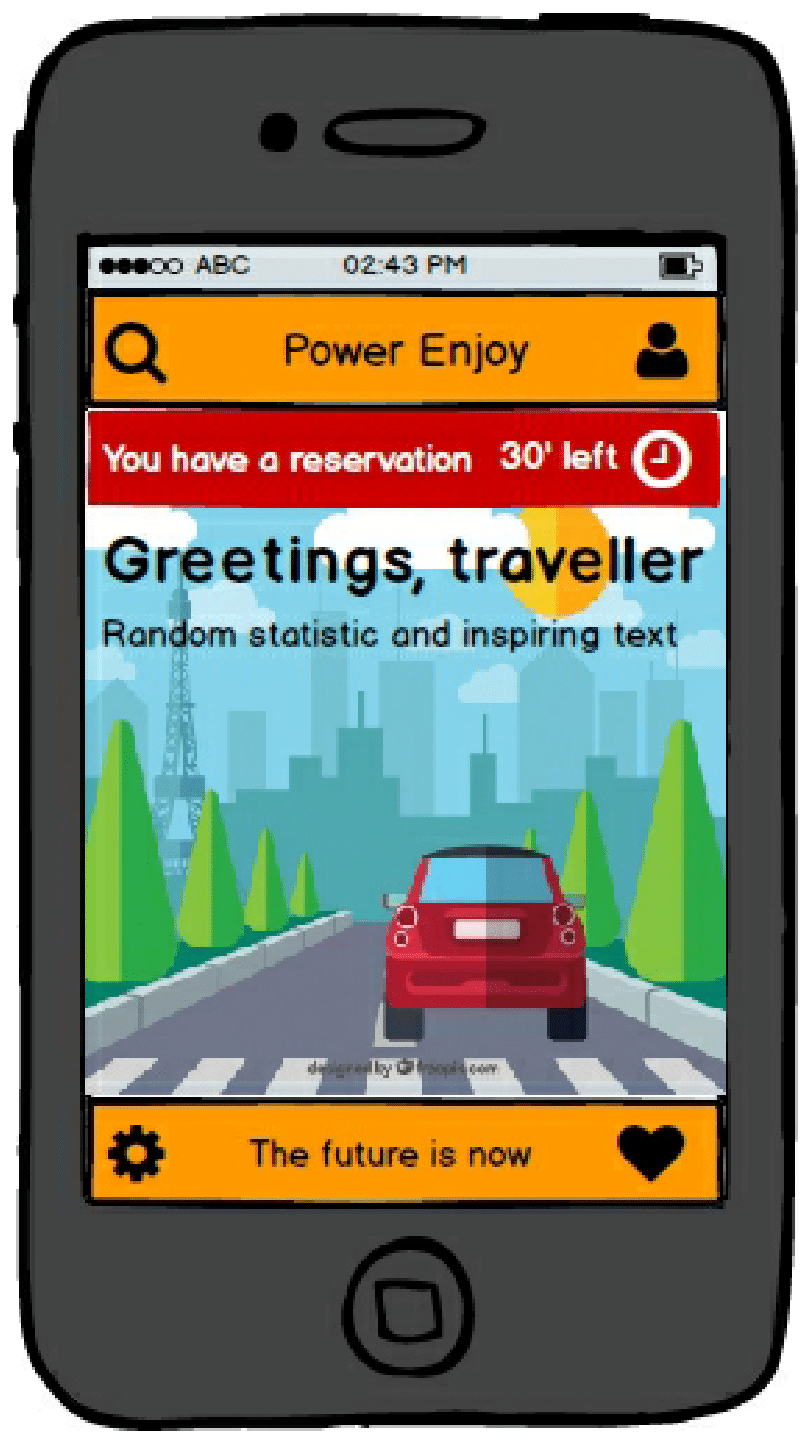
\includegraphics[width=1.56250in]{./MobileApp/MobileApp-1.png}
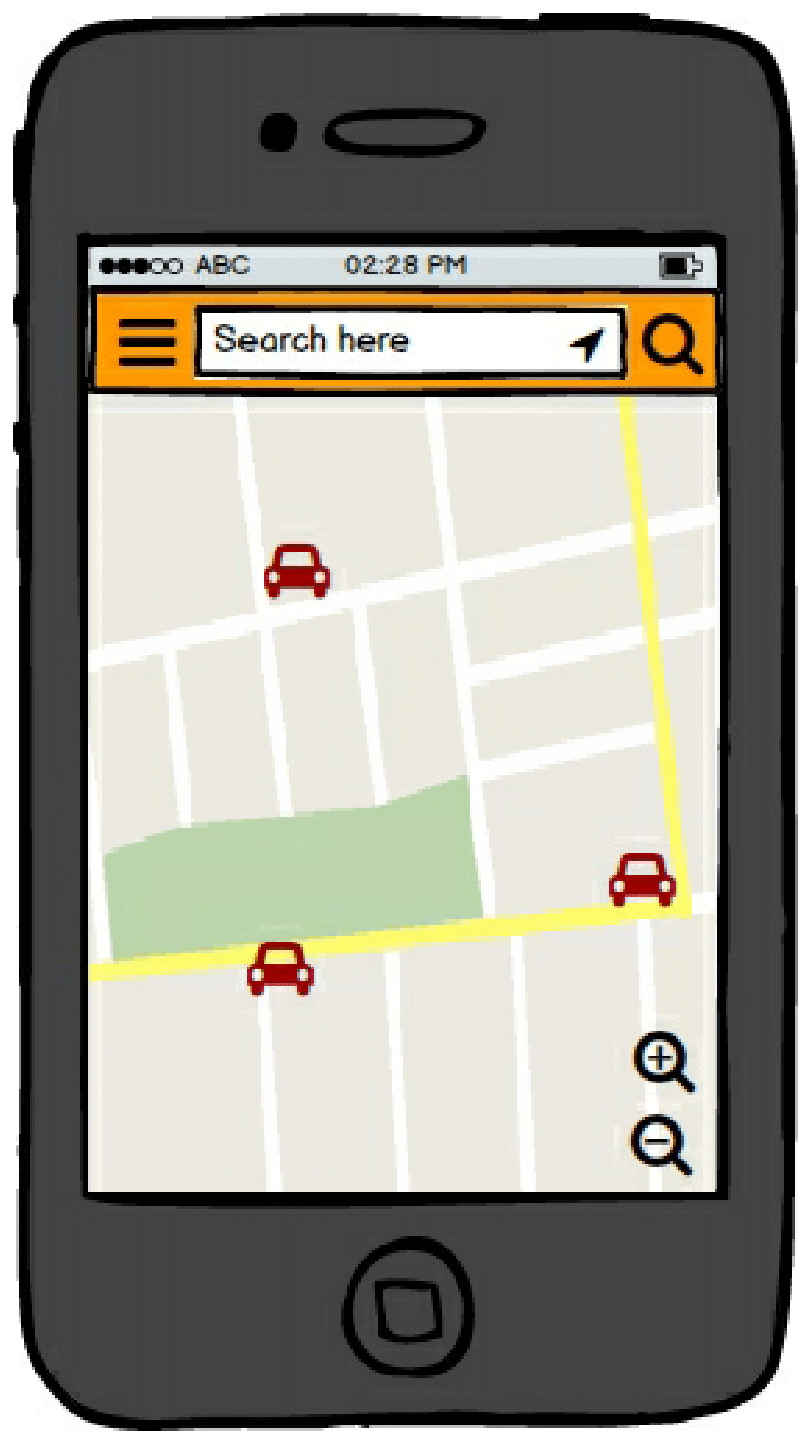
\includegraphics[width=1.56250in]{./MobileApp/MobileApp-2.png}
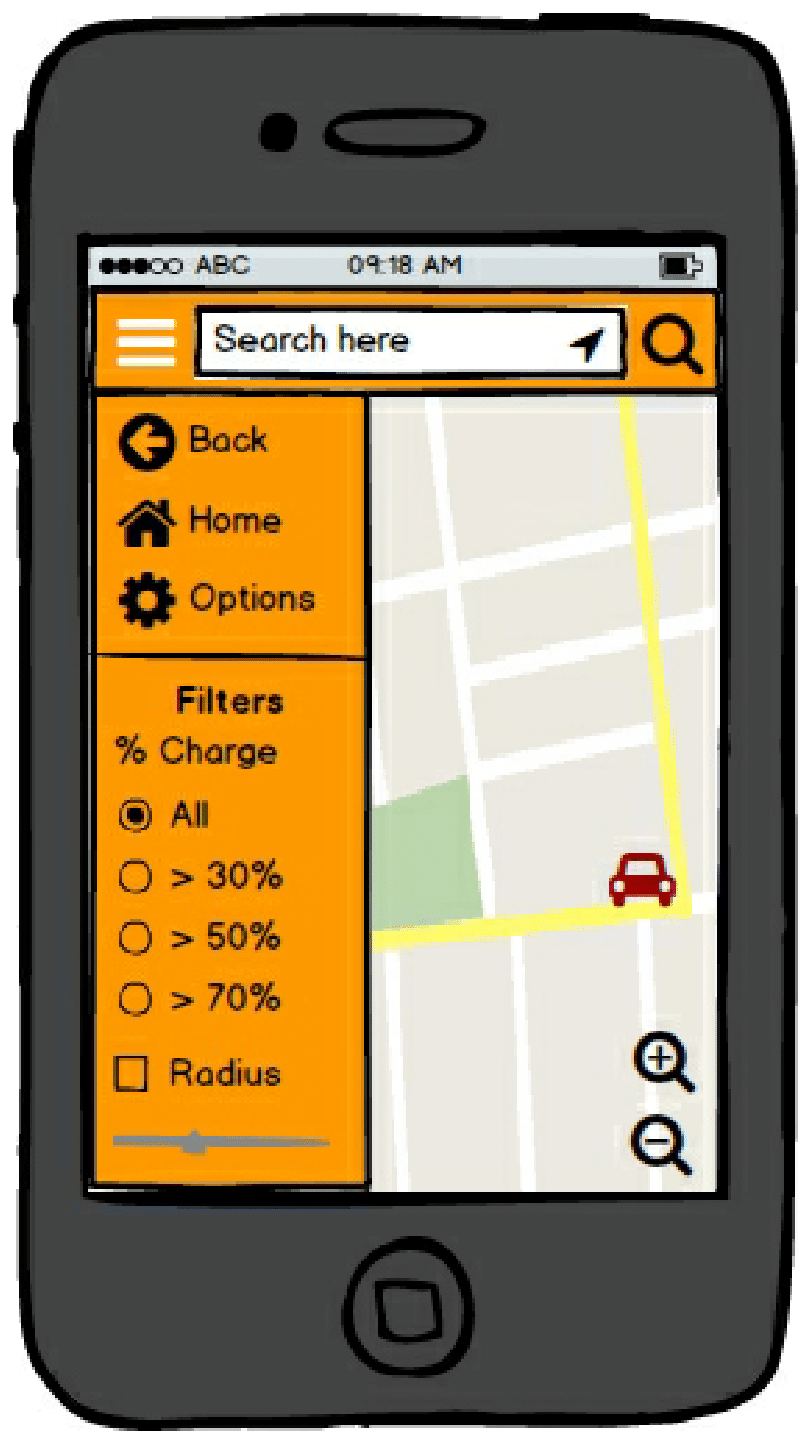
\includegraphics[width=1.56250in]{./MobileApp/MobileApp-3.png}
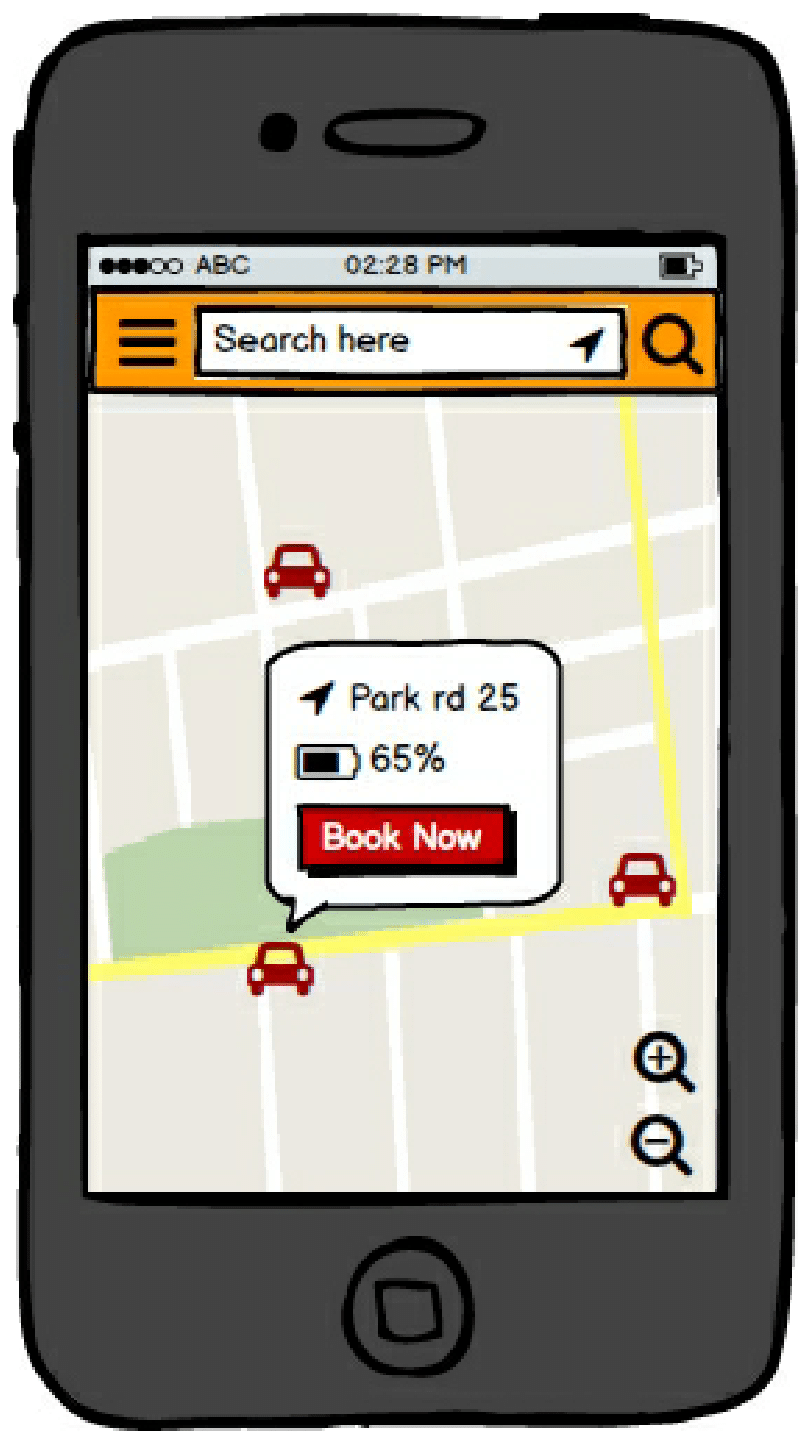
\includegraphics[width=1.56250in]{./MobileApp/MobileApp-4.png}
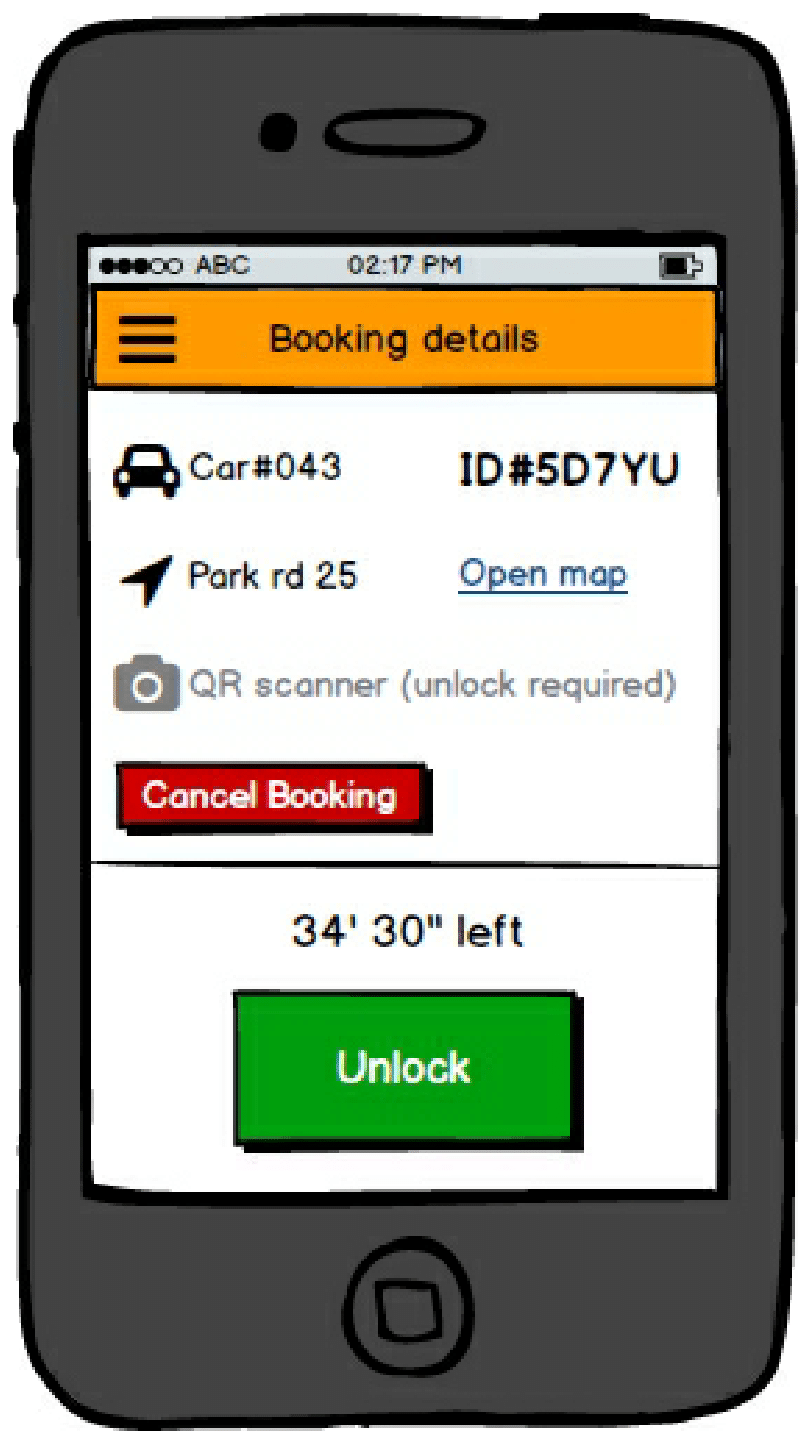
\includegraphics[width=1.56250in]{./MobileApp/MobileApp-5.png}
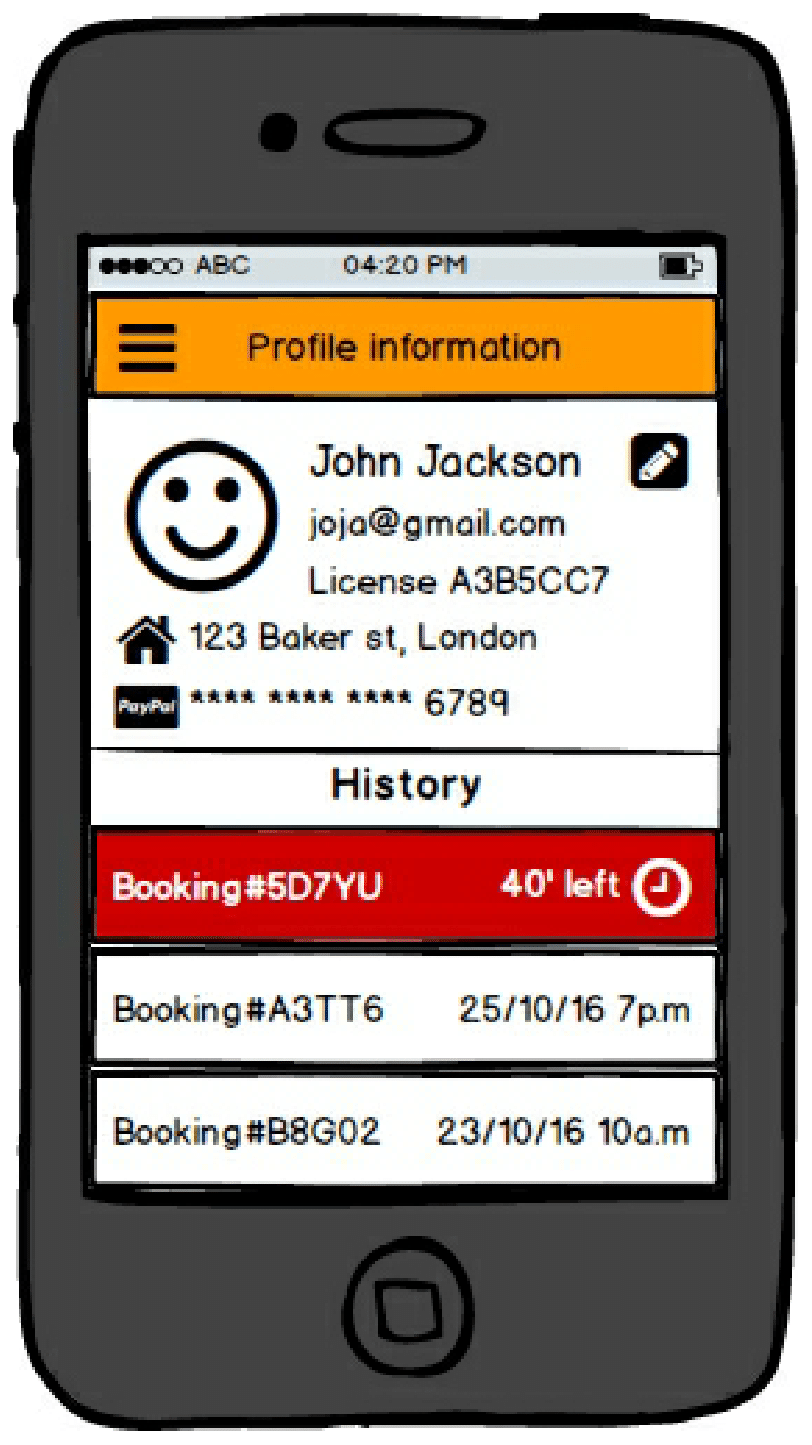
\includegraphics[width=1.56250in]{./MobileApp/MobileApp-6.png} \newpage

\subparagraph{\texorpdfstring{Car system
\newline \newline}{Car system }}\label{car-system}

\centerline{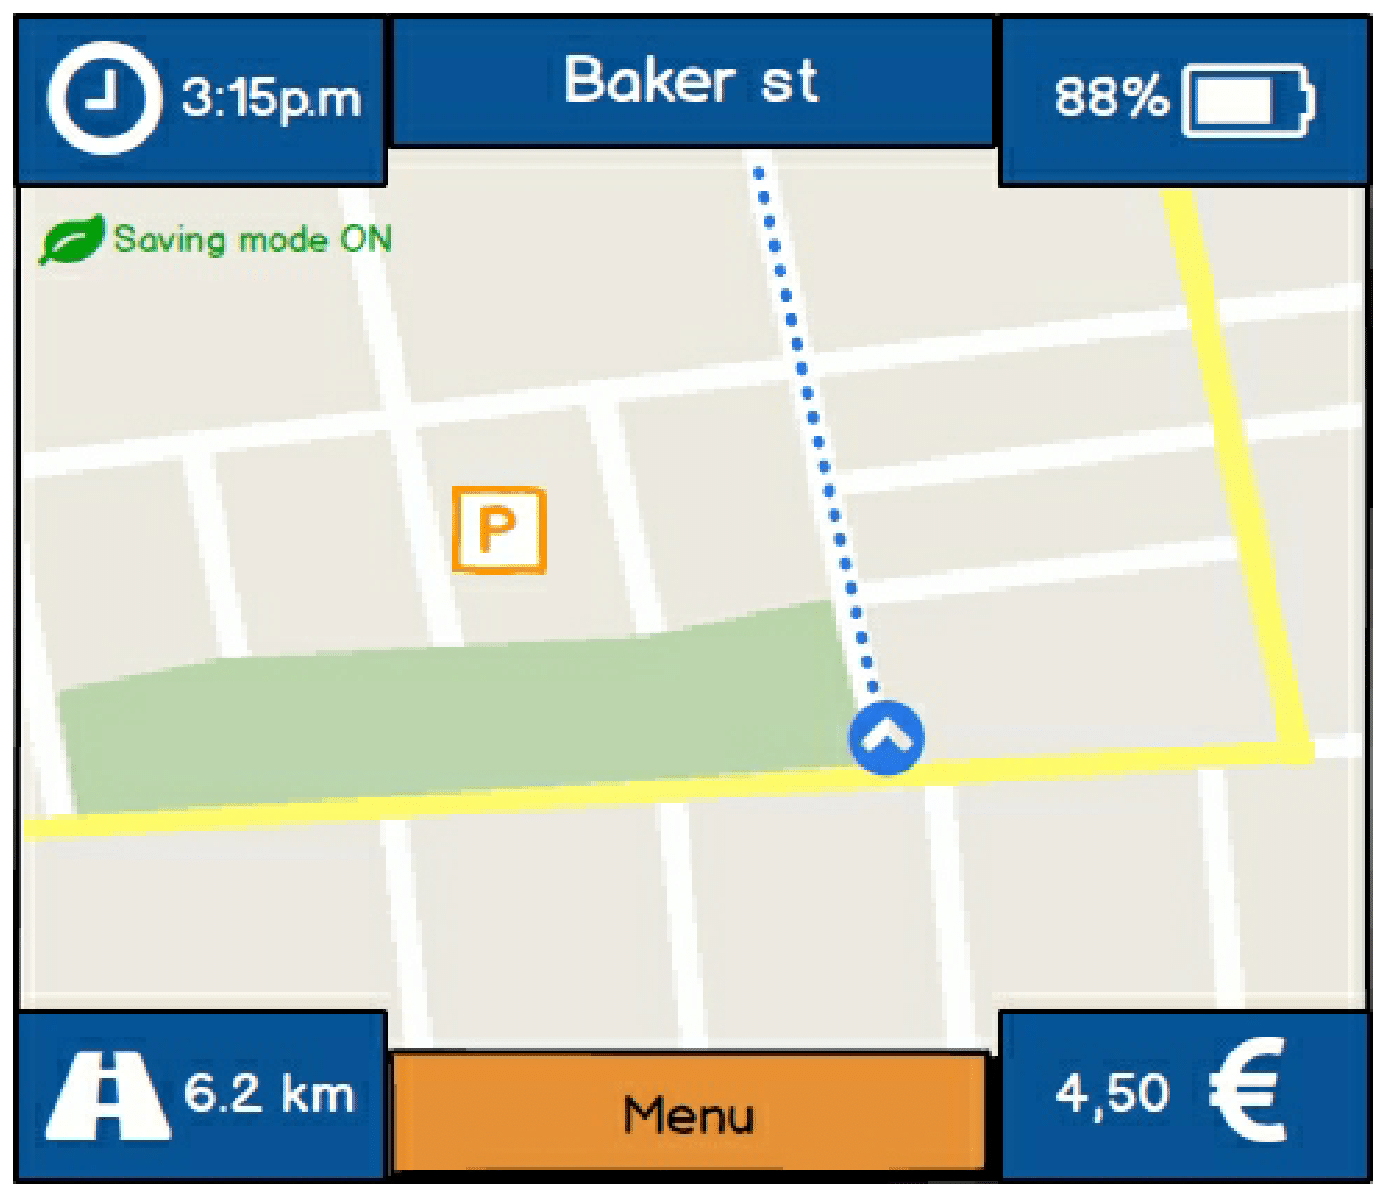
\includegraphics[width=3.12500in]{./CarSystem/CarSystem-1.png}}

\centerline{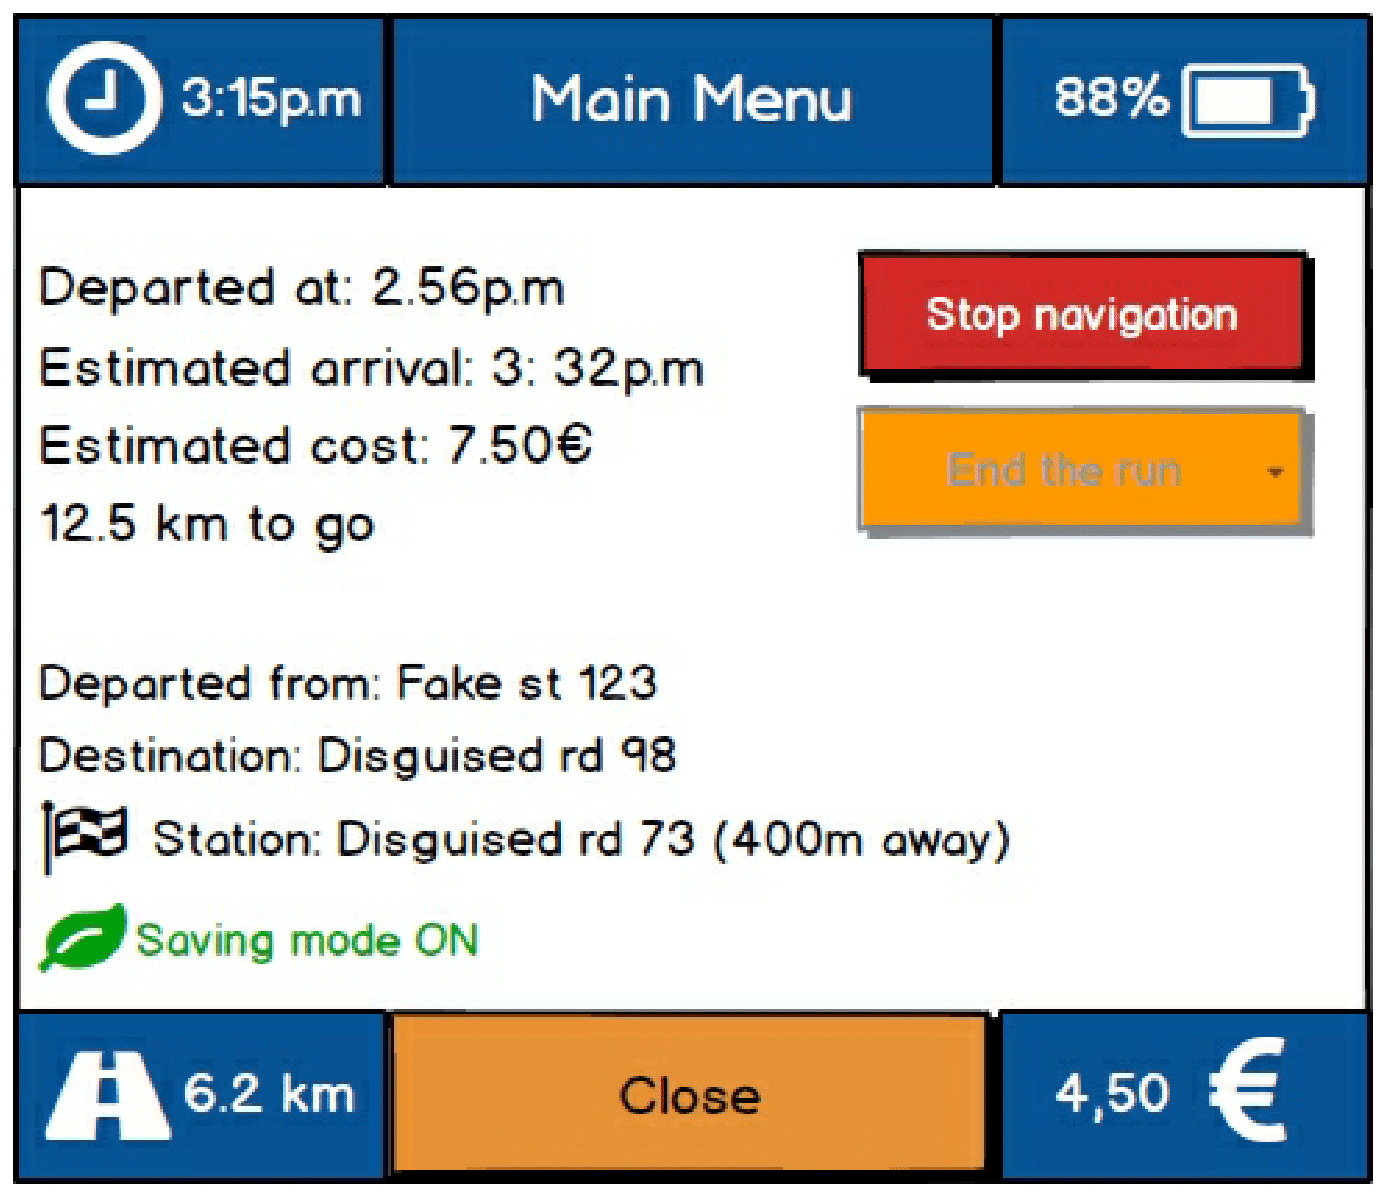
\includegraphics[width=3.12500in]{./CarSystem/CarSystem-2.png}}\newpage

\subparagraph{\texorpdfstring{Monitoring service
\newline \newline}{Monitoring service }}\label{monitoring-service}

\centerline{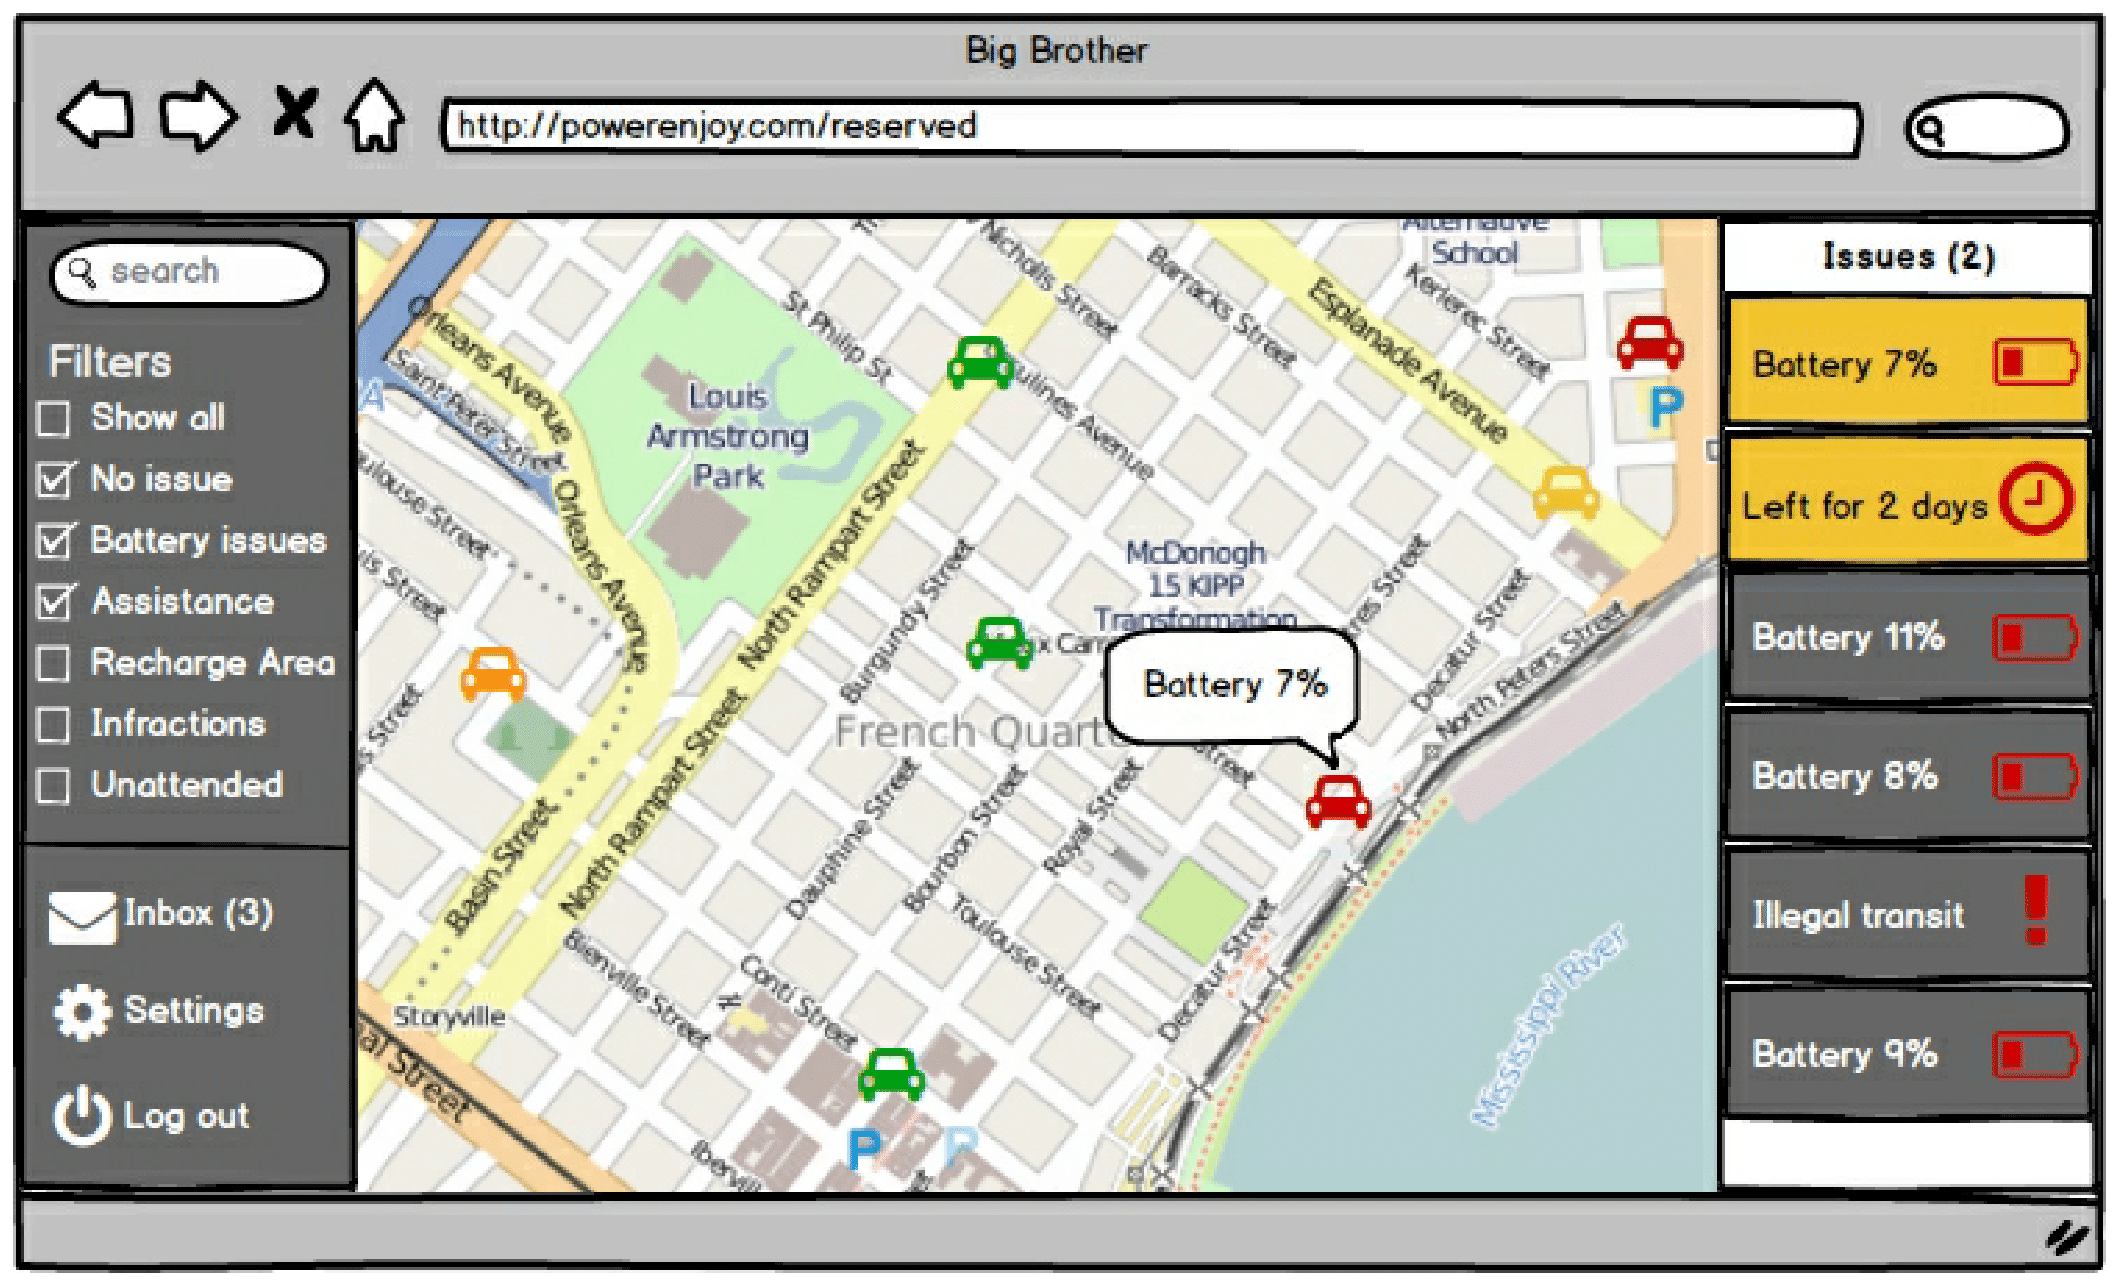
\includegraphics[width=4.16667in]{./Monitoringservice/Monitoringservice-1.png}}

\centerline{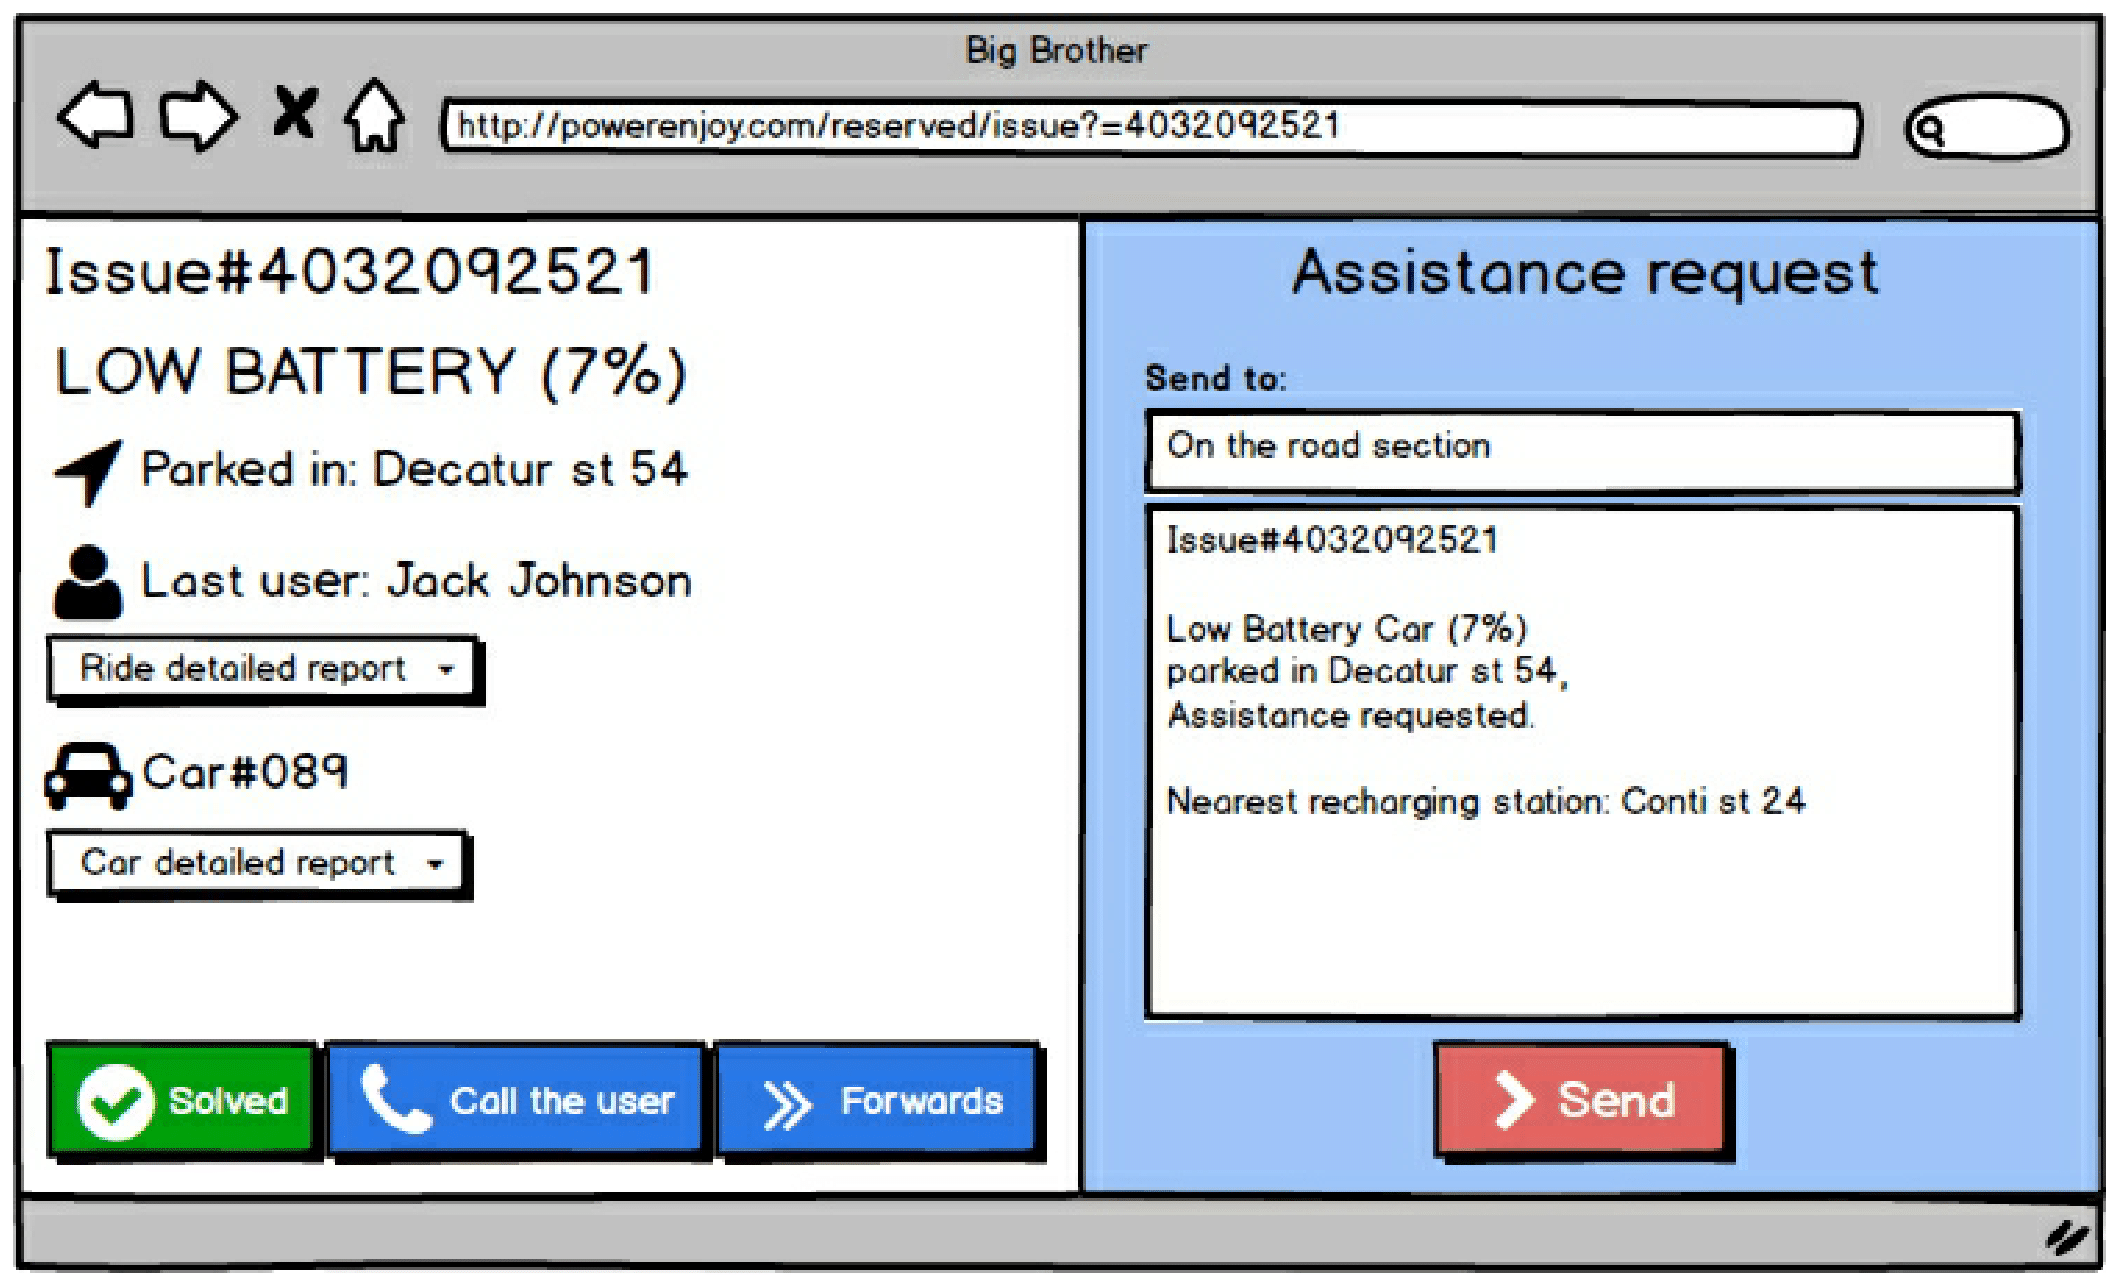
\includegraphics[width=4.16667in]{./Monitoringservice/Monitoringservice-2.png}}\newpage

\subsection{9 Scenario identifying}\label{scenario-identifying}

Here are listed some different scenarios of our system to be usage.

\subsubsection{Scenario 1}\label{scenario-1}

Ted is running late for a job interview since the bus engine failed, so
he opens the PowerEnJoy mobile application and searches for an available
car around his current position within a radius of 700 meters. He finds
that the nearest car is just 250 meters away, so he clicks the icon on
the map corresponding to the chosen car and looks through the details
screen; the car has 30\% battery left but his destination is not far and
from the estimation provided in the details he thinks the can make it,
so he hits the ``reserve'' button, he drops off the bus and starts
walking towards the car guided by the GPS. Arrived to the car, Ted
clicks the ``Open Car'' button and enters the vehicle. Once inside the
system asks Ted to scan the QR code on the car screen with the QR
scanner featured in the PowerEnJoy application. Once recognized, Ted is
free to power up the car and start his ride. When Ted arrives to his
destination he powers down the car and gets an on screen notification
saying that he has driven more than 2 kilometers, the car has less than
the 20\% of battery left and there isn't any recharging station within 3
kilometers from his position, therefore he can take the car closer to
the recharging station and get a discount or leave there the vehicle but
this will cost him an increased fare. Ted has no time to move the car so
he decides to pay the penalty, he exits the car and the system takes
care of locking it. The ride is successfully completed and Ted is
charged for the right amount of money on his PayPal account.

\subsubsection{Scenario 2}\label{scenario-2}

Gwen has invited some friends over for dinner, while eating they decide
to go out for a beer later, so Gwen decides to book a car with the
PowerEnJoy application, John and Paula, her two friends, are not
registered to the service yet; since Gwen wants to save money by taking
two registered users with her, she asks them to download the application
on their smartphone and proceed with the registration. Once opened the
application they're asked if they want to login or to register, they
choose the second and then insert valid credentials and receive their
password via e-mail. Finished the dinner they go out, unfortunately Gwen
forgets her driving license at home so they have to go back to get it
and by the time they're back the reservation time expires and Gwen is
charged with a fine for not having picked up the car in time. They
proceed to book the same car again, since no other has done it in the
meantime, get to it and step inside. Now the three scan the QR code with
their smartphones and the system notifies Gwen that a discount will be
applied on the cost of the trip. Once at destination they drop off the
car and the system sends a notification warning that she left the car in
a non safe area and therefore she has to keep paying with a reduced fare
and must get back to the car in at most two hours. They are ok with that
and walk inside the pub, again they loose track of time until Gwen's
phone rings as she gets notified that two hours passed and she's getting
to pay for them plus another fine for improper use of the service.

\subsubsection{Scenario 3}\label{scenario-3}

Tony is preparing to go to his friend Matt, he's going to ride there
with Matt's bike which he borrowed a week ago so he can give it back to
him, after that they have to go to the shopping center at the boundaries
of the city, so Tony decides to book a PowerEnJoy car with the mobile
application. He inserts Matt's house address into the system and books
the most convenient car. Once at Matt's place the two go to pick the car
up, once they are inside and the check-in is done, they decide to select
the ``money saving option'', after inserting their destination the
system provides them a suitable recharging station to leave the car at.
Luckily for them the recharging station is inside the shopping center
area so, once parked, they power the car down and get out, once outside
they insert the plug in the specific socket and leave. The system
notifies Tony with the payment details including the applied discount.

\subsubsection{Scenario 4}\label{scenario-4}

Melanie, a PowerEnJoy operator, is working at her terminal, monitoring
the cars in her assigned area through the interface provided by the
PowerEnJoy system. She is checking through flagged cars which have low
battery level. The first she overviews has been recently used and is in
a central part of the city so she decides to leave it as it is, since
it's likely it will be used anyway. The second one is in a remote part
of the city and hasn't been picked up or booked since the previous day,
so she decides to send maintenance personal to recharge it. To do so she
enters the ``assistance request'' screen and starts to type in the
request details. While doing so she gets a push notification that warns
her about the urgent need of maintenance for a vehicle. Thanks to the
maintenance system integration she's able to quickly forward the request
to the specific facility which will take charge of it and therefore she
can go back to the request she was previously working on. After
successfully sending on the request she goes back to the analysis of the
flagged cars, until she gets another notification, this time the
notification reports that a user has improperly left a car for more than
two hours outside a safe parking area, she looks over the details and
finds out that the car is in the suburb of the town and so she decides
to ask for an operator to have it picked up and moved inside of a safe
area, again through the integrated system she's able to have a
maintenance operator to handle the request.

\subsubsection{Scenario 5}\label{scenario-5}

Bob, an operator of PowerEnJoy, has been assigned to update the system
terms regarding to a new company policy. First of all he modifies the
cost per minute for the service usage from 26 cents/minute to 28
cents/minute. The price raise is balanced with a proper increase in
discounts, so, still through the provided interface, Bob can increase
the discount, for leaving the car plugged in a charging station, from
25\% to 30\% on the full price of the ride. In the end Bob has to insert
two new safe areas and to remove one; the interface allows Bob to select
the proper utility and he can easily select, from the list of safe
areas, the one to delete. Now he inserts the first new area just by
specifying the chosen address and the radius around it, which in this
case is of 2.6 km. Since the second area has a more complicated shape he
selects the drawing tool and easily draws the polygon defining the
selected area, then the system commutates the area drew on the map into
proper coordinates to identify it. After this process Bob checks out the
update, the system generates a proper notification containing the new
terms and conditions document and the update details and therefore sends
it over to the users.

\newpage

\subsection{10 UML Models}\label{uml-models}

\subsubsection{10.1 Class Diagram}\label{class-diagram}

Relations between Boundaries, Coordinates and other classes are omitted
for clarity.\\
Discounts and penalties are calculated from the informations in the ride
and in the used car, and are part of the ``Details'' in the transaction
class.

\centerline{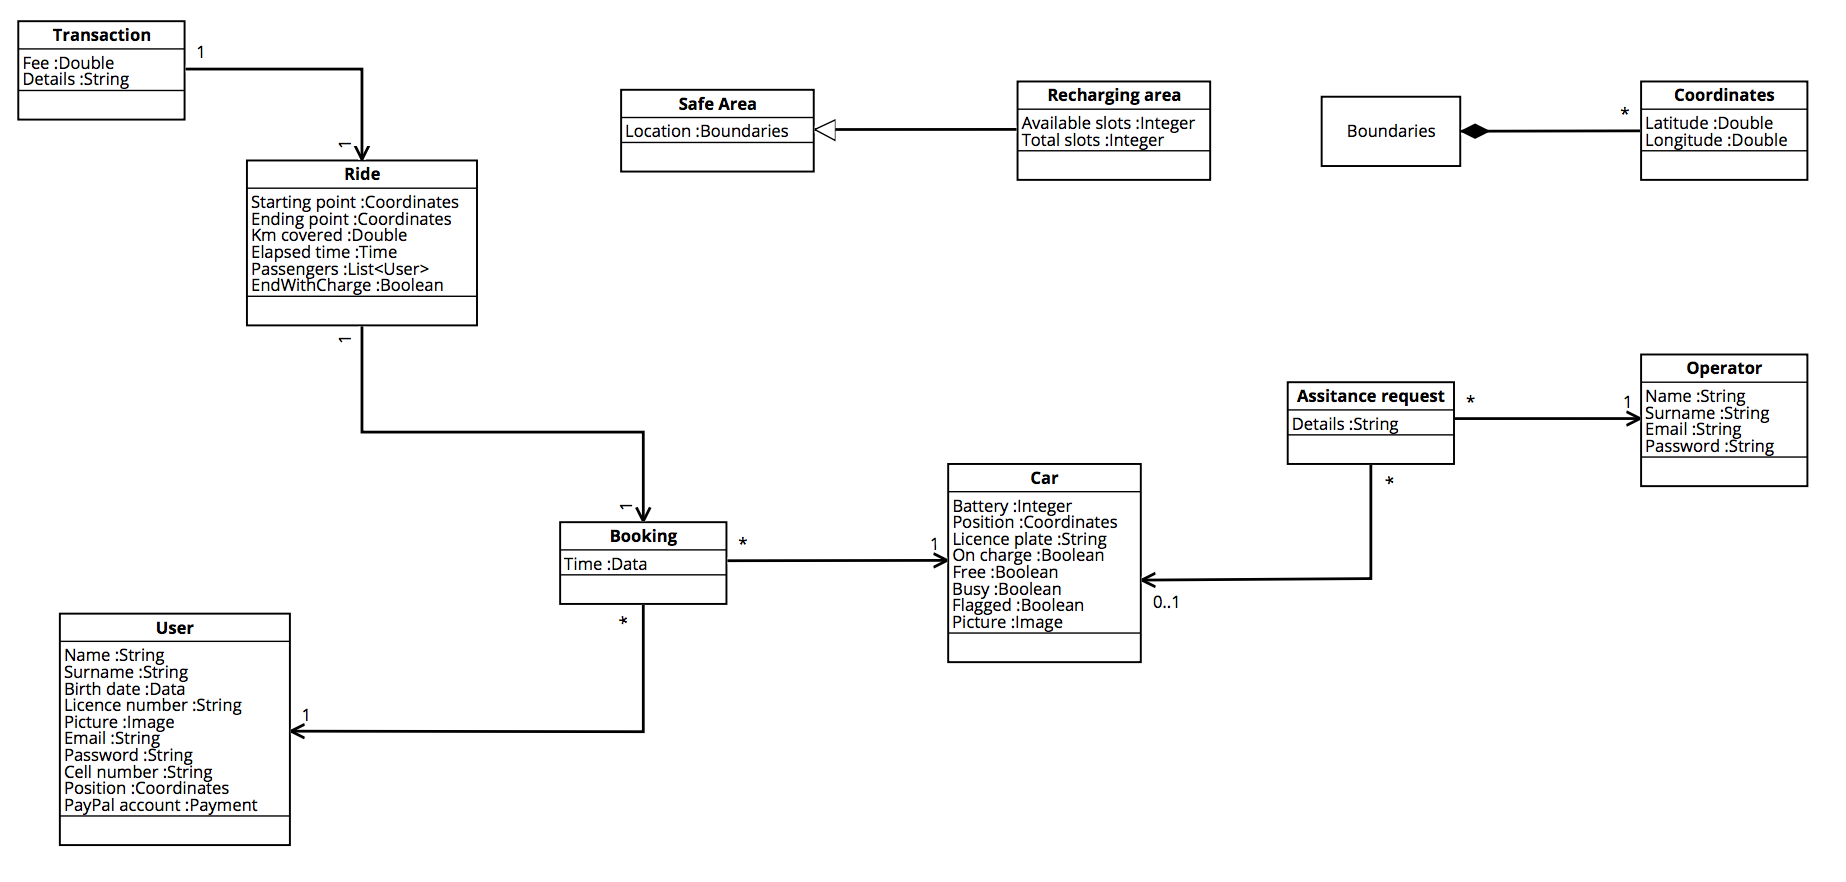
\includegraphics[width=6.25000in]{./classdiagram/classdiagram-1.png}}\newpage

\subsubsection{10.2 Use case diagram}\label{use-case-diagram}

\centerline{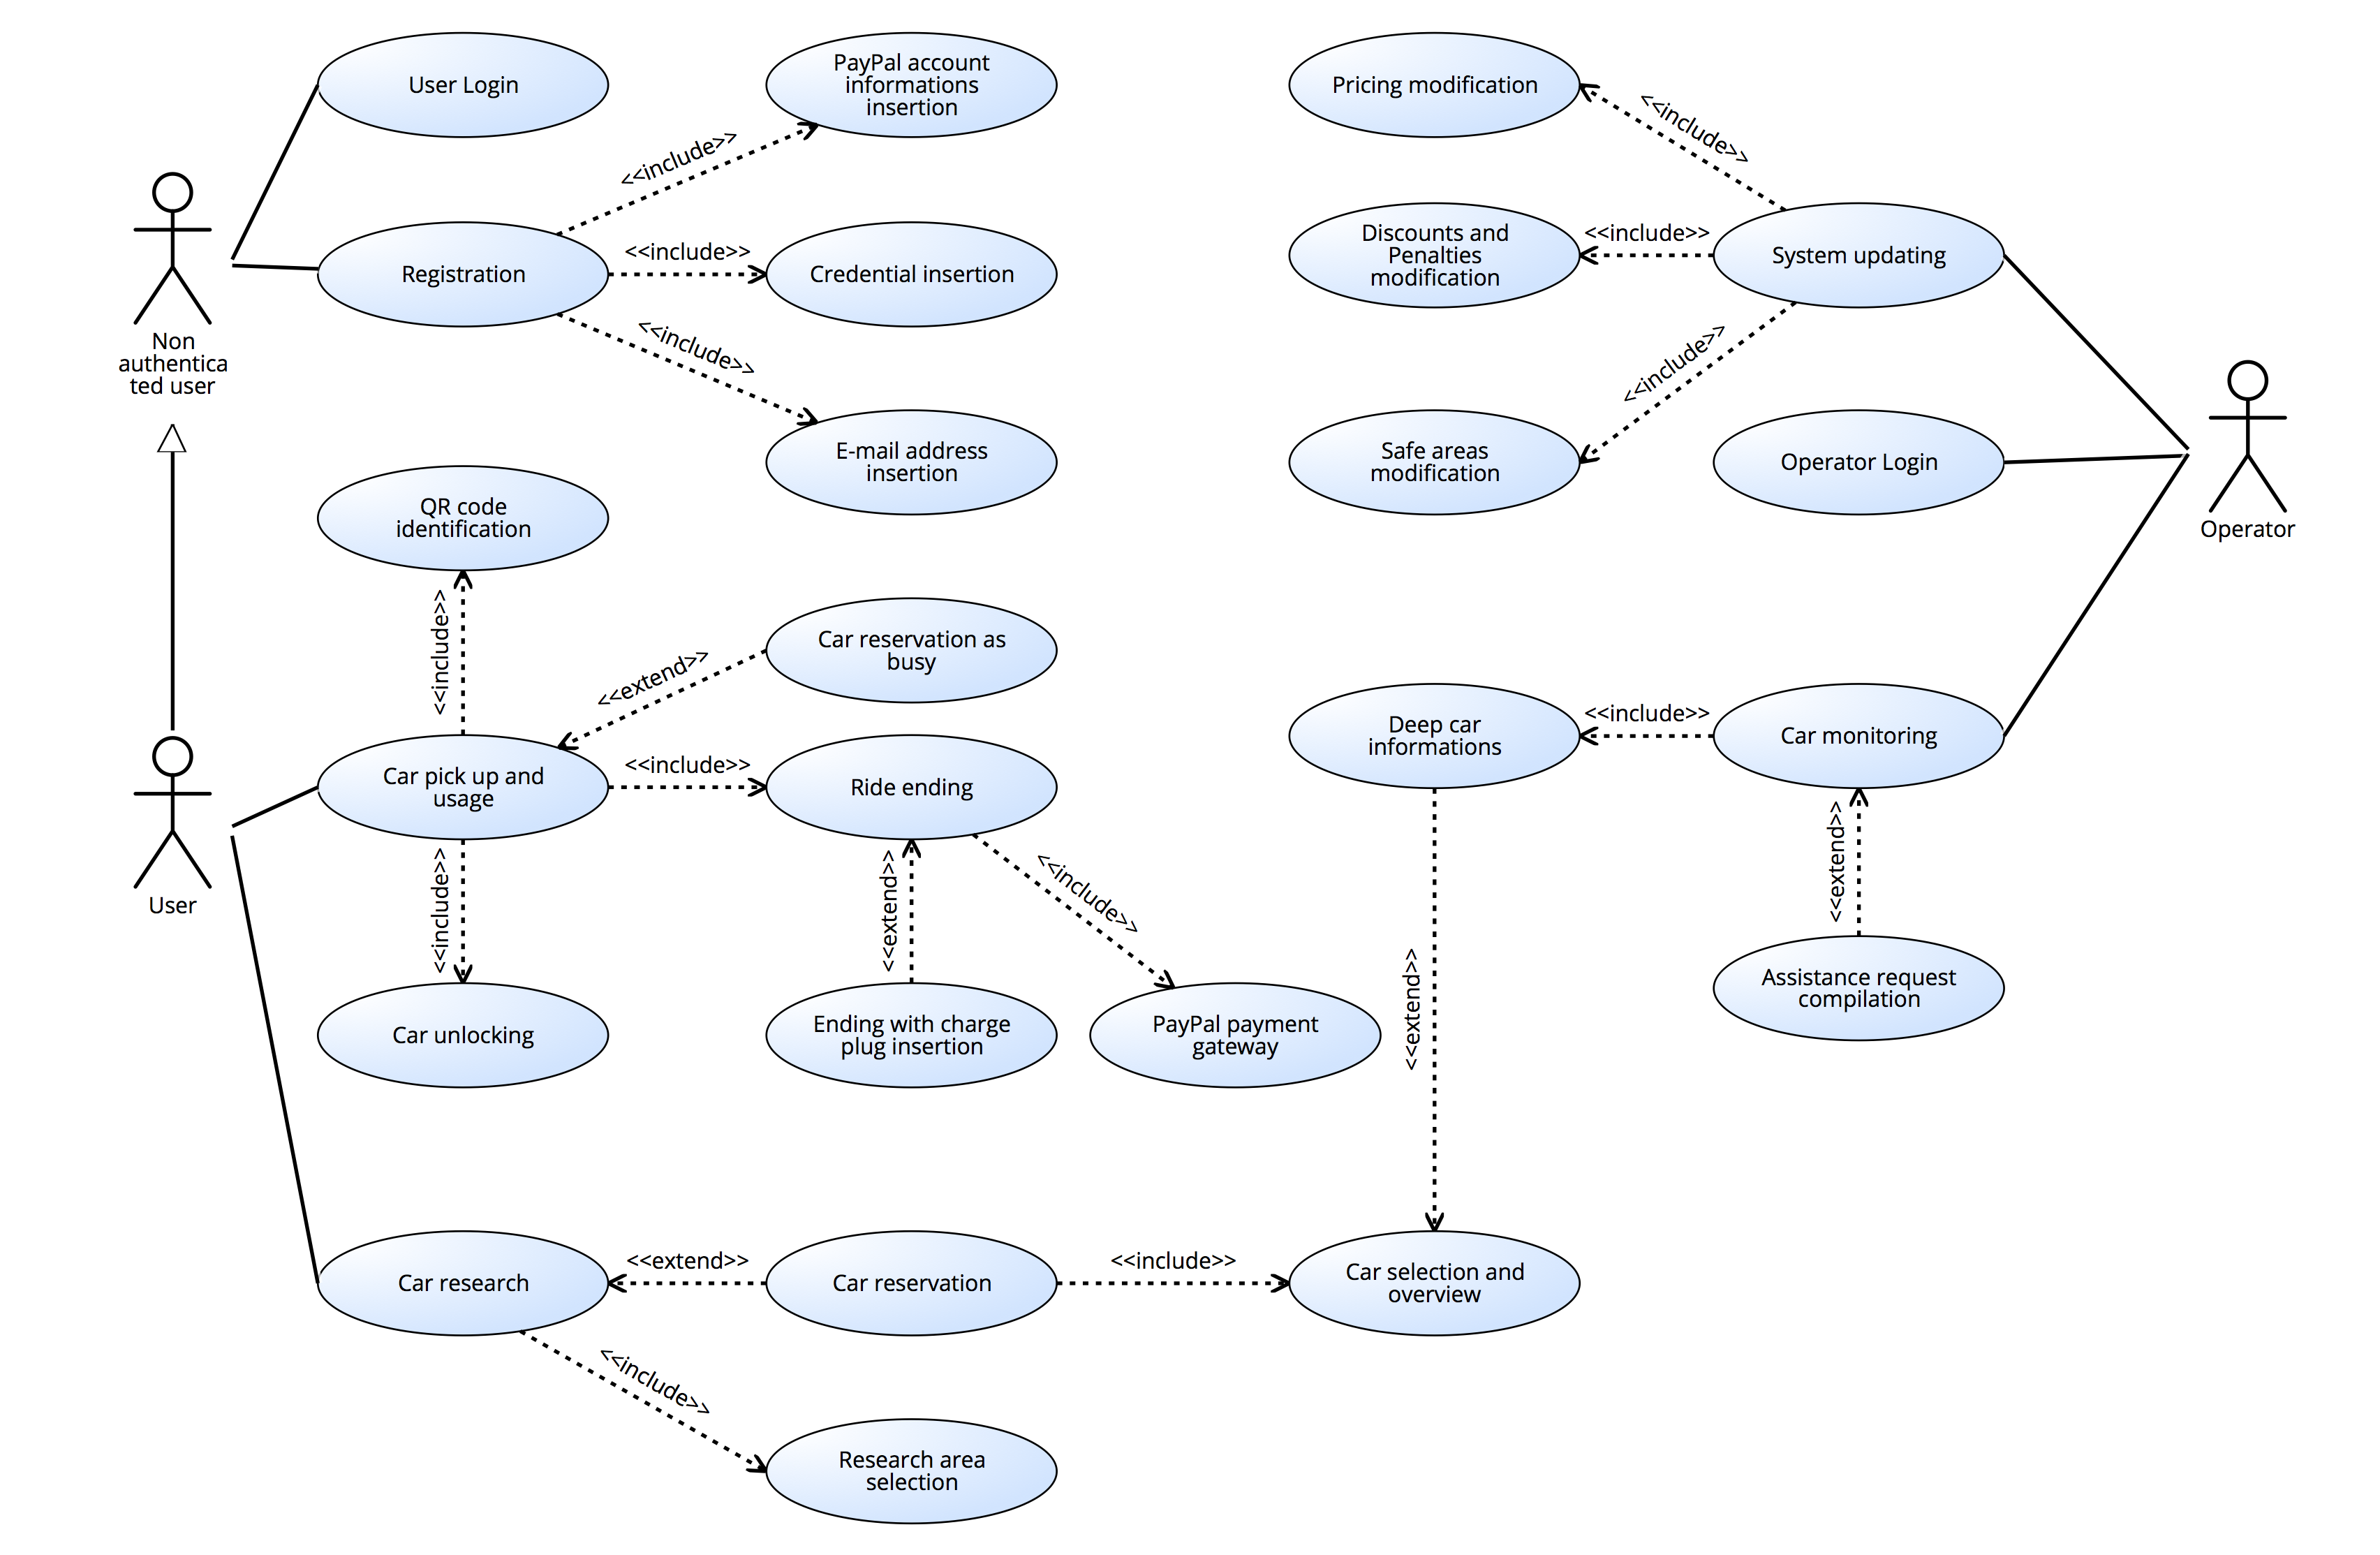
\includegraphics[width=6.25000in]{./uc/uc.png}}\newpage

\subsubsection{10.3 Use case description}\label{use-case-description}

In this section are listed some common or significant use cases
derivable from the Use Case diagram.

\paragraph{User logs in}\label{user-logs-in}

\begin{longtable}[]{@{}ll@{}}
\toprule
\begin{minipage}[t]{0.29\columnwidth}\raggedright\strut
\textbf{Name}\strut
\end{minipage} & \begin{minipage}[t]{0.65\columnwidth}\raggedright\strut
User logs in\strut
\end{minipage}\tabularnewline
\begin{minipage}[t]{0.29\columnwidth}\raggedright\strut
\textbf{Goals}\strut
\end{minipage} & \begin{minipage}[t]{0.65\columnwidth}\raggedright\strut
G0\strut
\end{minipage}\tabularnewline
\begin{minipage}[t]{0.29\columnwidth}\raggedright\strut
\textbf{Actors}\strut
\end{minipage} & \begin{minipage}[t]{0.65\columnwidth}\raggedright\strut
Non authenticated user\strut
\end{minipage}\tabularnewline
\begin{minipage}[t]{0.29\columnwidth}\raggedright\strut
\textbf{Entry conditions}\strut
\end{minipage} & \begin{minipage}[t]{0.65\columnwidth}\raggedright\strut
The user must be registered but hasn't logged on yet.\strut
\end{minipage}\tabularnewline
\begin{minipage}[t]{0.29\columnwidth}\raggedright\strut
\textbf{Flow of events}\strut
\end{minipage} & \begin{minipage}[t]{0.65\columnwidth}\raggedright\strut
\begin{itemize}
\tightlist
\item
  The user enters the login screen of the mobile application.
\item
  The user types in his username and his password.
\item
  The user taps on the ``Login'' button.
\item
  The user is redirected to the car research screen.
\end{itemize}\strut
\end{minipage}\tabularnewline
\begin{minipage}[t]{0.29\columnwidth}\raggedright\strut
\textbf{Exit conditions}\strut
\end{minipage} & \begin{minipage}[t]{0.65\columnwidth}\raggedright\strut
The user is redirected on the car research screen.\strut
\end{minipage}\tabularnewline
\begin{minipage}[t]{0.29\columnwidth}\raggedright\strut
\textbf{Exceptions}\strut
\end{minipage} & \begin{minipage}[t]{0.65\columnwidth}\raggedright\strut
The username and the password are not a valid couple. If this happens
the system doesn't allow the user to enter the research screen, however
he's notified of the incorrectness of the credentials and therefore is
kept on the login screen to try again.\strut
\end{minipage}\tabularnewline
\bottomrule
\end{longtable}

\newpage

\subparagraph{\texorpdfstring{Login Sequence
Diagram\newline}{Login Sequence Diagram}}\label{login-sequence-diagram}

\centerline{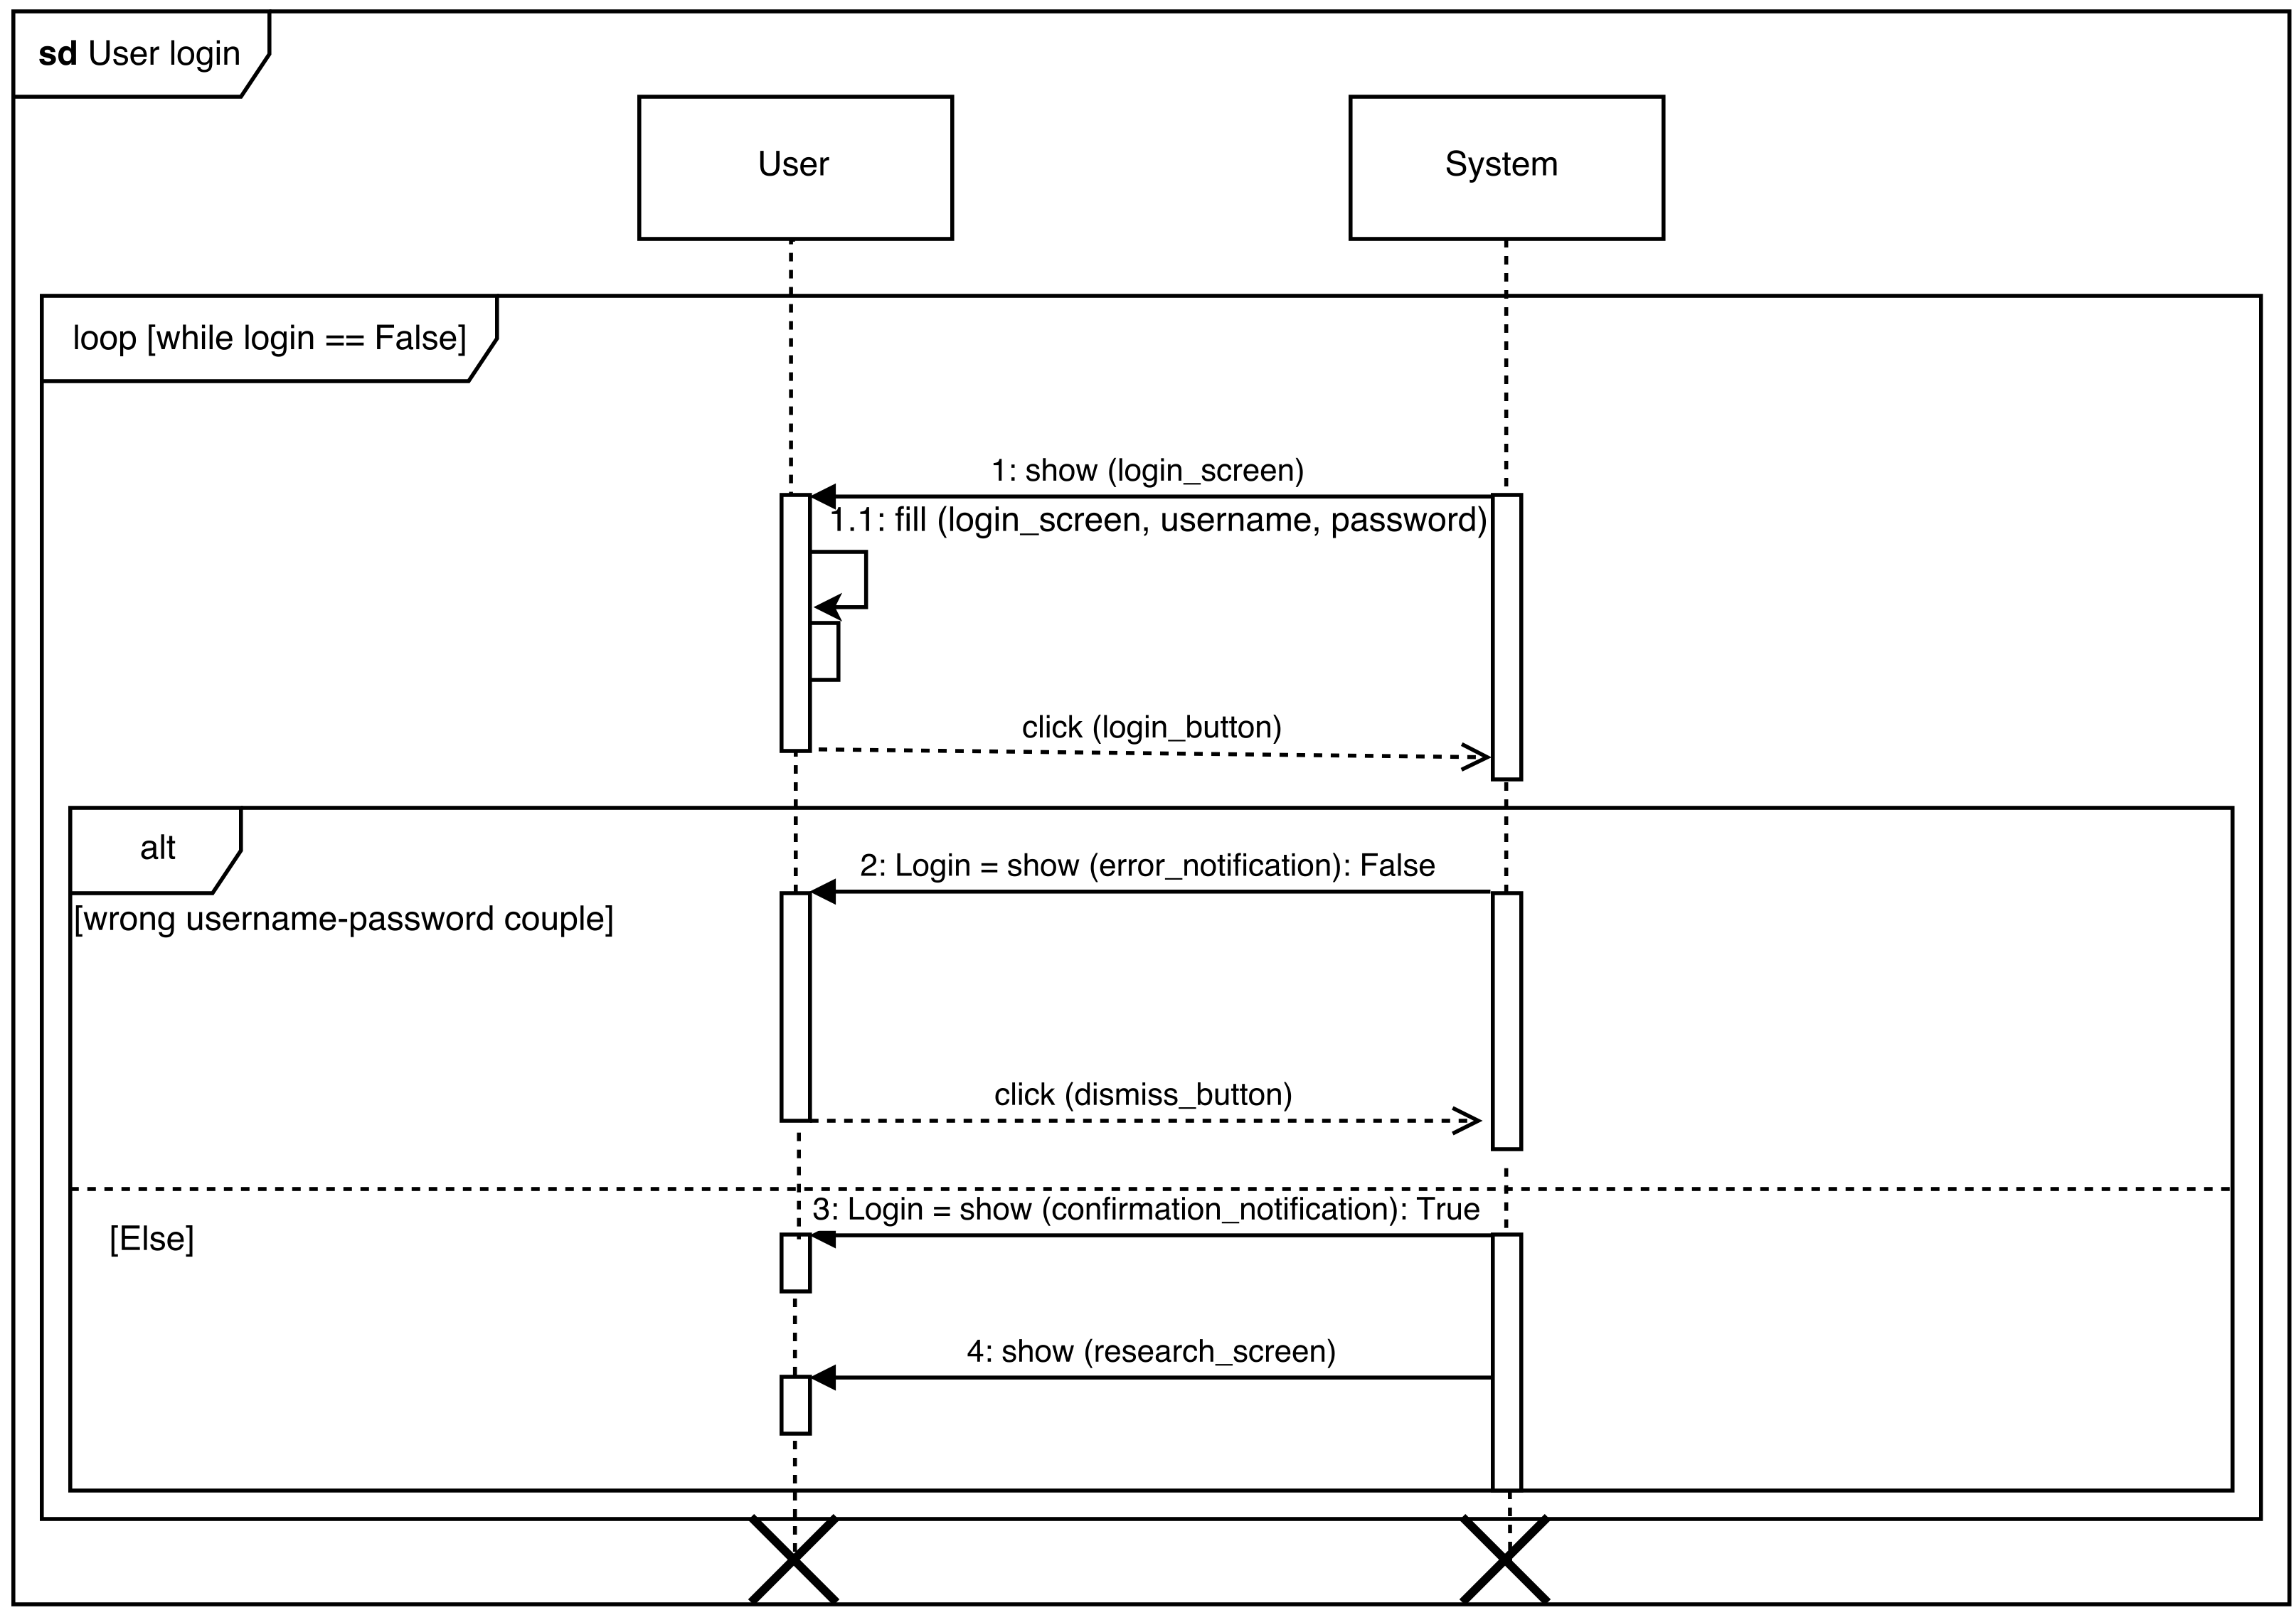
\includegraphics[width=6.25000in]{./FlowDiagrams/UserLoginSD.png}}

\newpage

\paragraph{User registers}\label{user-registers}

\begin{longtable}[]{@{}ll@{}}
\toprule
\begin{minipage}[t]{0.29\columnwidth}\raggedright\strut
\textbf{Name}\strut
\end{minipage} & \begin{minipage}[t]{0.65\columnwidth}\raggedright\strut
User registers\strut
\end{minipage}\tabularnewline
\begin{minipage}[t]{0.29\columnwidth}\raggedright\strut
\textbf{Goals}\strut
\end{minipage} & \begin{minipage}[t]{0.65\columnwidth}\raggedright\strut
G0\strut
\end{minipage}\tabularnewline
\begin{minipage}[t]{0.29\columnwidth}\raggedright\strut
\textbf{Actors}\strut
\end{minipage} & \begin{minipage}[t]{0.65\columnwidth}\raggedright\strut
Non authenticated user\strut
\end{minipage}\tabularnewline
\begin{minipage}[t]{0.29\columnwidth}\raggedright\strut
\textbf{Entry conditions}\strut
\end{minipage} & \begin{minipage}[t]{0.65\columnwidth}\raggedright\strut
The user is not registered to the service yet.\strut
\end{minipage}\tabularnewline
\begin{minipage}[t]{0.29\columnwidth}\raggedright\strut
\textbf{Flow of events}\strut
\end{minipage} & \begin{minipage}[t]{0.65\columnwidth}\raggedright\strut
\begin{itemize}
\tightlist
\item
  The user enters the login screen of the mobile application.
\item
  The user taps on the ``Register'' button.
\item
  The user is redirected to the credential insertion screen.
\item
  The user inserts his name, surname, birth date and driving license ID
  in any order.
\item
  The user taps on the ``Next'' button.
\item
  The user is redirected to the PayPal account insertion screen.
\item
  The user inputs his PayPal credentials.
\item
  The user taps on the ``Next'' button.
\item
  The user is redirected to the e-mail insertion screen.
\item
  The user types in an e-mail address.
\item
  The user taps on the ``Confirm'' button.
\item
  The system sends a confirmation message to the specified e-mail
  address.
\item
  The user is redirected to a screen informing him to check is e-mail.
\item
  The user clicks on the link contained in the sent e-mail.
\item
  The system activates the new user's account.
\item
  The user is redirected into the mobile application inside a successful
  registration screen.
\item
  The user taps on the ``Confirm'' button.
\item
  The user is redirected to the car research screen.
\end{itemize}\strut
\end{minipage}\tabularnewline
\begin{minipage}[t]{0.29\columnwidth}\raggedright\strut
\textbf{Exit conditions}\strut
\end{minipage} & \begin{minipage}[t]{0.65\columnwidth}\raggedright\strut
The user is registered and is redirected to the car research
screen.\strut
\end{minipage}\tabularnewline
\begin{minipage}[t]{0.29\columnwidth}\raggedright\strut
\textbf{Exceptions}\strut
\end{minipage} & \begin{minipage}[t]{0.65\columnwidth}\raggedright\strut
The user inserts invalid PayPal credentials or license ID, personal
information do not match license credentials, license or e-mail address
are already bounded to an existing profile. In this case the user is
notified of the error and is redirected to the login screen.\strut
\end{minipage}\tabularnewline
\bottomrule
\end{longtable}

\newpage

\paragraph{User searches and reserves a
car}\label{user-searches-and-reserves-a-car}

\begin{longtable}[]{@{}ll@{}}
\toprule
\begin{minipage}[t]{0.29\columnwidth}\raggedright\strut
\textbf{Name}\strut
\end{minipage} & \begin{minipage}[t]{0.65\columnwidth}\raggedright\strut
User searches and reserves a car\strut
\end{minipage}\tabularnewline
\begin{minipage}[t]{0.29\columnwidth}\raggedright\strut
\textbf{Goals}\strut
\end{minipage} & \begin{minipage}[t]{0.65\columnwidth}\raggedright\strut
G1, G2\strut
\end{minipage}\tabularnewline
\begin{minipage}[t]{0.29\columnwidth}\raggedright\strut
\textbf{Actors}\strut
\end{minipage} & \begin{minipage}[t]{0.65\columnwidth}\raggedright\strut
User\strut
\end{minipage}\tabularnewline
\begin{minipage}[t]{0.29\columnwidth}\raggedright\strut
\textbf{Entry conditions}\strut
\end{minipage} & \begin{minipage}[t]{0.65\columnwidth}\raggedright\strut
The user is logged in the mobile application.\strut
\end{minipage}\tabularnewline
\begin{minipage}[t]{0.29\columnwidth}\raggedright\strut
\textbf{Flow of events}\strut
\end{minipage} & \begin{minipage}[t]{0.65\columnwidth}\raggedright\strut
\begin{itemize}
\tightlist
\item
  The user enters the car research screen.
\item
  The user types in an address or chooses to use his GPS location.
\item
  The user hits the ``Search'' button.
\item
  The system shows in the map all the available cars in the selected
  location
\item
  The user clicks on the chosen car.
\item
  The system shows a pop-up with the car informations.
\item
  The user hits the ``Book now'' button.
\item
  The user is redirected to the booking details page, showing the time
  left before the reservation expires.
\end{itemize}\strut
\end{minipage}\tabularnewline
\begin{minipage}[t]{0.29\columnwidth}\raggedright\strut
\textbf{Exit conditions}\strut
\end{minipage} & \begin{minipage}[t]{0.65\columnwidth}\raggedright\strut
The car is correctly reserved and the user is redirected to the map
screen.\strut
\end{minipage}\tabularnewline
\begin{minipage}[t]{0.29\columnwidth}\raggedright\strut
\textbf{Exceptions}\strut
\end{minipage} & \begin{minipage}[t]{0.65\columnwidth}\raggedright\strut
The chosen car is no more available. In this case the user is notified
of the error and redirected to the map screen.\strut
\end{minipage}\tabularnewline
\bottomrule
\end{longtable}

\newpage

\subparagraph{Booking Sequence Diagram}\label{booking-sequence-diagram}

\centerline{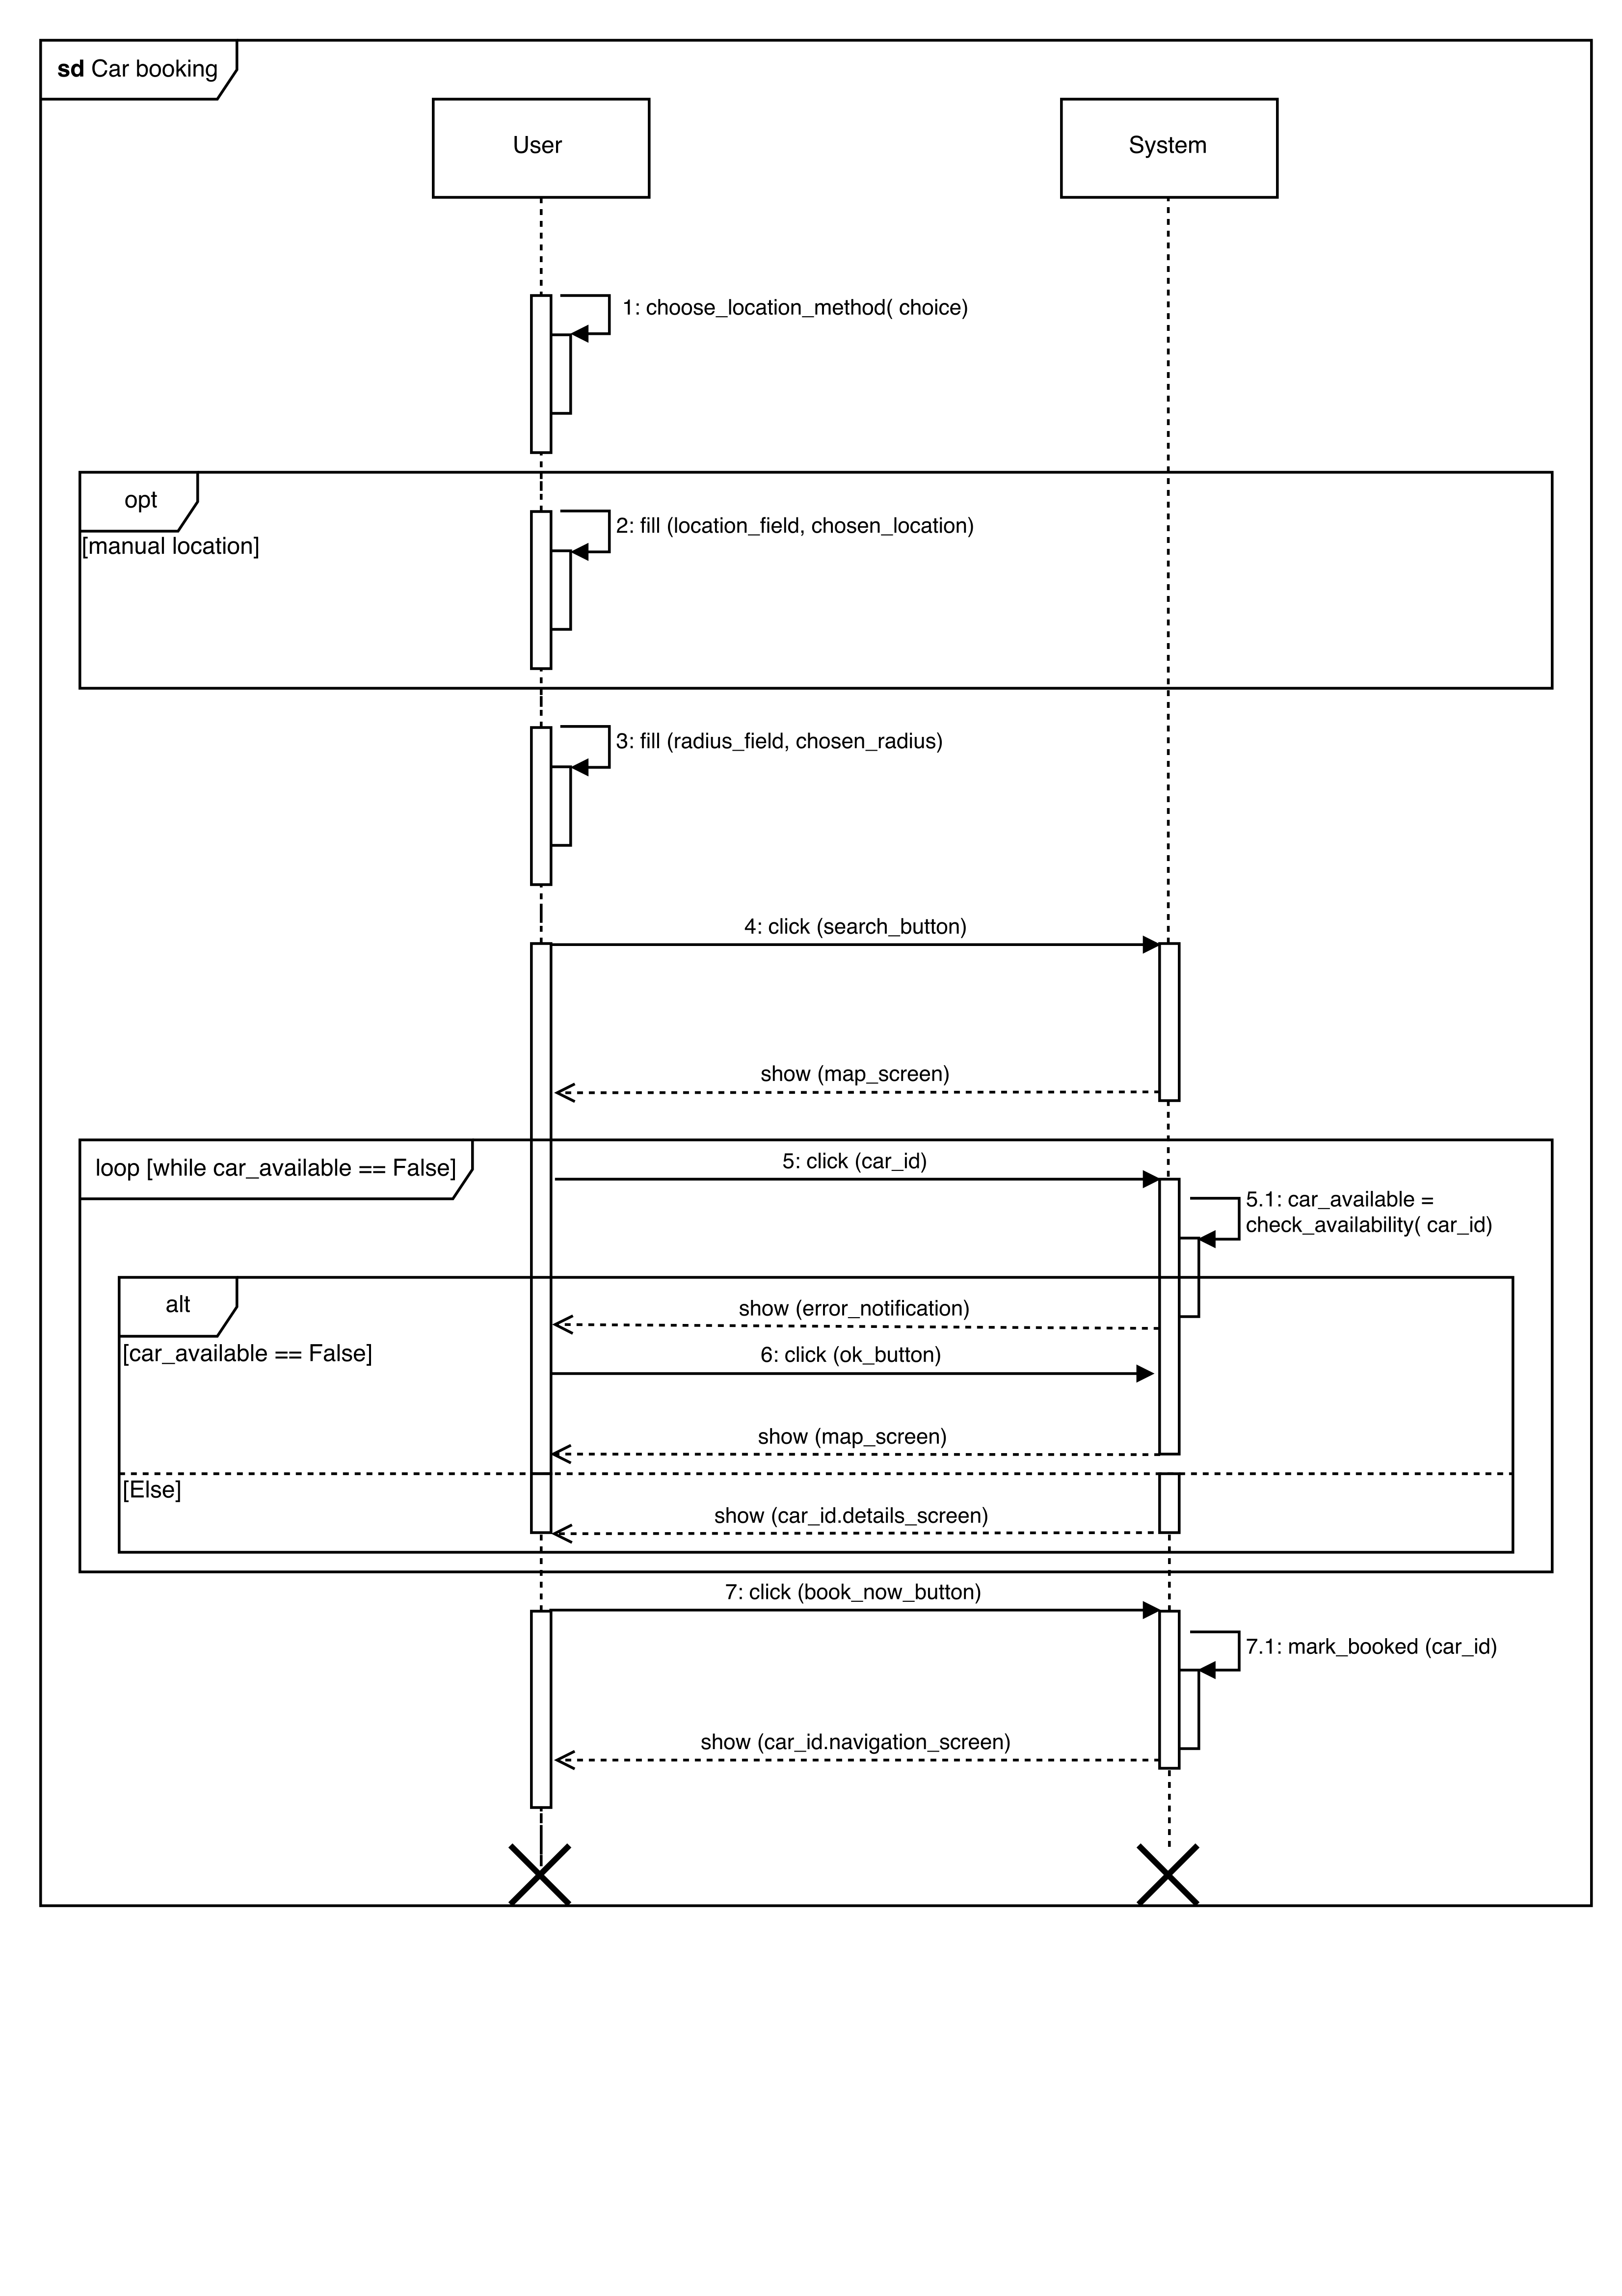
\includegraphics[width=5.20833in]{./FlowDiagrams/CarBookingSD.png}}\newpage

\paragraph{User picks the car up}\label{user-picks-the-car-up}

\begin{longtable}[]{@{}ll@{}}
\toprule
\begin{minipage}[t]{0.29\columnwidth}\raggedright\strut
\textbf{Name}\strut
\end{minipage} & \begin{minipage}[t]{0.65\columnwidth}\raggedright\strut
User picks the car up\strut
\end{minipage}\tabularnewline
\begin{minipage}[t]{0.29\columnwidth}\raggedright\strut
\textbf{Goals}\strut
\end{minipage} & \begin{minipage}[t]{0.65\columnwidth}\raggedright\strut
G2\strut
\end{minipage}\tabularnewline
\begin{minipage}[t]{0.29\columnwidth}\raggedright\strut
\textbf{Actors}\strut
\end{minipage} & \begin{minipage}[t]{0.65\columnwidth}\raggedright\strut
User\strut
\end{minipage}\tabularnewline
\begin{minipage}[t]{0.29\columnwidth}\raggedright\strut
\textbf{Entry conditions}\strut
\end{minipage} & \begin{minipage}[t]{0.65\columnwidth}\raggedright\strut
The user made a reservation for the car he's about to pick up.\strut
\end{minipage}\tabularnewline
\begin{minipage}[t]{0.29\columnwidth}\raggedright\strut
\textbf{Flow of events}\strut
\end{minipage} & \begin{minipage}[t]{0.65\columnwidth}\raggedright\strut
\begin{itemize}
\tightlist
\item
  The user enters his profile screen.
\item
  The user hits the car reservation inside the history tab.
\item
  The user is redirected to the reservation details screen.
\item
  The user touches the ``Unlock'' button.
\item
  The system unlocks the car.
\item
  The user enters the car.
\item
  The Car screen power on.
\item
  The user clicks on the QR scanner button.
\item
  The user scans the QR code on the car screen.
\item
  The user powers the engine by pressing the physical button inside the
  car.
\end{itemize}\strut
\end{minipage}\tabularnewline
\begin{minipage}[t]{0.29\columnwidth}\raggedright\strut
\textbf{Exit conditions}\strut
\end{minipage} & \begin{minipage}[t]{0.65\columnwidth}\raggedright\strut
The user checked in and the car is powered up.\strut
\end{minipage}\tabularnewline
\begin{minipage}[t]{0.29\columnwidth}\raggedright\strut
\textbf{Exceptions}\strut
\end{minipage} & \begin{minipage}[t]{0.65\columnwidth}\raggedright\strut
\begin{itemize}
\tightlist
\item
  The user unlocks the car but doesn't power it up in 15 minutes. If
  this happens then the car is marked as free and locked up again.
\end{itemize}\strut
\end{minipage}\tabularnewline
\bottomrule
\end{longtable}

\newpage

\paragraph{User starts a ride with money saving
option}\label{user-starts-a-ride-with-money-saving-option}

\begin{longtable}[]{@{}ll@{}}
\toprule
\begin{minipage}[t]{0.29\columnwidth}\raggedright\strut
\textbf{Name}\strut
\end{minipage} & \begin{minipage}[t]{0.65\columnwidth}\raggedright\strut
User starts a ride with money saving option\strut
\end{minipage}\tabularnewline
\begin{minipage}[t]{0.29\columnwidth}\raggedright\strut
\textbf{Goals}\strut
\end{minipage} & \begin{minipage}[t]{0.65\columnwidth}\raggedright\strut
G4, G5\strut
\end{minipage}\tabularnewline
\begin{minipage}[t]{0.29\columnwidth}\raggedright\strut
\textbf{Actors}\strut
\end{minipage} & \begin{minipage}[t]{0.65\columnwidth}\raggedright\strut
User\strut
\end{minipage}\tabularnewline
\begin{minipage}[t]{0.29\columnwidth}\raggedright\strut
\textbf{Entry conditions}\strut
\end{minipage} & \begin{minipage}[t]{0.65\columnwidth}\raggedright\strut
User checked in and powered up the car.\strut
\end{minipage}\tabularnewline
\begin{minipage}[t]{0.29\columnwidth}\raggedright\strut
\textbf{Flow of events}\strut
\end{minipage} & \begin{minipage}[t]{0.65\columnwidth}\raggedright\strut
\begin{itemize}
\tightlist
\item
  The user clicks the ``Money saving'' button on the car screen.
\item
  The car shows the destination insertion screen.
\item
  The user inserts his destination and hits the ``Confirm'' button.
\item
  The system calculates the optimal charge station.
\item
  The car monitor show the GPS navigation map screen with the selected
  charge station as destination.
\item
  The user starts his ride.
\end{itemize}\strut
\end{minipage}\tabularnewline
\begin{minipage}[t]{0.29\columnwidth}\raggedright\strut
\textbf{Exit conditions}\strut
\end{minipage} & \begin{minipage}[t]{0.65\columnwidth}\raggedright\strut
The user is riding the car and the car screen shows the navigation
towards the desired destination.\strut
\end{minipage}\tabularnewline
\begin{minipage}[t]{0.29\columnwidth}\raggedright\strut
\textbf{Exceptions}\strut
\end{minipage} & \begin{minipage}[t]{0.65\columnwidth}\raggedright\strut
In the case there's no compatible charging station the user is
redirected to a screen notifying the problem and then back to the
initial car screen.\strut
\end{minipage}\tabularnewline
\bottomrule
\end{longtable}

\newpage

\paragraph{The user parks and keeps the car as
busy}\label{the-user-parks-and-keeps-the-car-as-busy}

\begin{longtable}[]{@{}ll@{}}
\toprule
\begin{minipage}[t]{0.29\columnwidth}\raggedright\strut
\textbf{Name}\strut
\end{minipage} & \begin{minipage}[t]{0.65\columnwidth}\raggedright\strut
The user parks and keeps the car as busy\strut
\end{minipage}\tabularnewline
\begin{minipage}[t]{0.29\columnwidth}\raggedright\strut
\textbf{Goals}\strut
\end{minipage} & \begin{minipage}[t]{0.65\columnwidth}\raggedright\strut
G2\strut
\end{minipage}\tabularnewline
\begin{minipage}[t]{0.29\columnwidth}\raggedright\strut
\textbf{Actors}\strut
\end{minipage} & \begin{minipage}[t]{0.65\columnwidth}\raggedright\strut
User\strut
\end{minipage}\tabularnewline
\begin{minipage}[t]{0.29\columnwidth}\raggedright\strut
\textbf{Entry conditions}\strut
\end{minipage} & \begin{minipage}[t]{0.65\columnwidth}\raggedright\strut
The user picked the car up and is riding it.\strut
\end{minipage}\tabularnewline
\begin{minipage}[t]{0.29\columnwidth}\raggedright\strut
\textbf{Flow of events}\strut
\end{minipage} & \begin{minipage}[t]{0.65\columnwidth}\raggedright\strut
\begin{itemize}
\tightlist
\item
  The user parks the car and powers down the engine.
\item
  The user is redirected to the ride ending screen.
\item
  The user selects the ``Keep as busy'' button.
\item
  The user exits the car and closes the car door.
\item
  The system locks the car.
\item
  The user enters his profile screen.
\item
  The user hits the busy car reservation inside the history tab.
\item
  The user is redirected to the reservation details screen.
\item
  The user hits the ``Unlock'' button.
\end{itemize}\strut
\end{minipage}\tabularnewline
\begin{minipage}[t]{0.29\columnwidth}\raggedright\strut
\textbf{Exit conditions}\strut
\end{minipage} & \begin{minipage}[t]{0.65\columnwidth}\raggedright\strut
The user picked up the car again.\strut
\end{minipage}\tabularnewline
\begin{minipage}[t]{0.29\columnwidth}\raggedright\strut
\textbf{Exceptions}\strut
\end{minipage} & \begin{minipage}[t]{0.65\columnwidth}\raggedright\strut
The user doesn't unlock the car before two hours passed from the moment
he made the car busy. In this case the car is marked as free and the
user is charged for the extra time the car was kept eccupied plus a fine
if the car was left outside a safe area.\strut
\end{minipage}\tabularnewline
\bottomrule
\end{longtable}

\newpage

\paragraph{User ends a ride}\label{user-ends-a-ride}

\begin{longtable}[]{@{}ll@{}}
\toprule
\begin{minipage}[t]{0.29\columnwidth}\raggedright\strut
\textbf{Name}\strut
\end{minipage} & \begin{minipage}[t]{0.65\columnwidth}\raggedright\strut
User ends a ride\strut
\end{minipage}\tabularnewline
\begin{minipage}[t]{0.29\columnwidth}\raggedright\strut
\textbf{Goals}\strut
\end{minipage} & \begin{minipage}[t]{0.65\columnwidth}\raggedright\strut
G3\strut
\end{minipage}\tabularnewline
\begin{minipage}[t]{0.29\columnwidth}\raggedright\strut
\textbf{Actors}\strut
\end{minipage} & \begin{minipage}[t]{0.65\columnwidth}\raggedright\strut
User\strut
\end{minipage}\tabularnewline
\begin{minipage}[t]{0.29\columnwidth}\raggedright\strut
\textbf{Entry conditions}\strut
\end{minipage} & \begin{minipage}[t]{0.65\columnwidth}\raggedright\strut
The user parked the car which is still powered on.\strut
\end{minipage}\tabularnewline
\begin{minipage}[t]{0.29\columnwidth}\raggedright\strut
\textbf{Flow of events}\strut
\end{minipage} & \begin{minipage}[t]{0.65\columnwidth}\raggedright\strut
\begin{itemize}
\tightlist
\item
  The user powers down the engine.
\item
  The car monitor show the ride ending screen.
\item
  The user selects the ``End ride'' button.
\item
  The user exits the car and closes the car door.
\item
  The system calculates the fare for the ride.
\item
  The user is charged for the service usage.
\end{itemize}\strut
\end{minipage}\tabularnewline
\begin{minipage}[t]{0.29\columnwidth}\raggedright\strut
\textbf{Exit conditions}\strut
\end{minipage} & \begin{minipage}[t]{0.65\columnwidth}\raggedright\strut
The car is free and the user is charged with the amount due.\strut
\end{minipage}\tabularnewline
\begin{minipage}[t]{0.29\columnwidth}\raggedright\strut
\textbf{Exceptions}\strut
\end{minipage} & \begin{minipage}[t]{0.65\columnwidth}\raggedright\strut
\begin{itemize}
\tightlist
\item
  At the end of the ride the user has not enough money to pay on his
  PayPal account. If that's the case then the payment will be kept as
  pending and during this time the user will be banned and will be
  unable to use the service.
\end{itemize}\strut
\end{minipage}\tabularnewline
\bottomrule
\end{longtable}

\newpage

\subparagraph{\texorpdfstring{Ride Activity Diagram
\newline}{Ride Activity Diagram }}\label{ride-activity-diagram}

\centerline{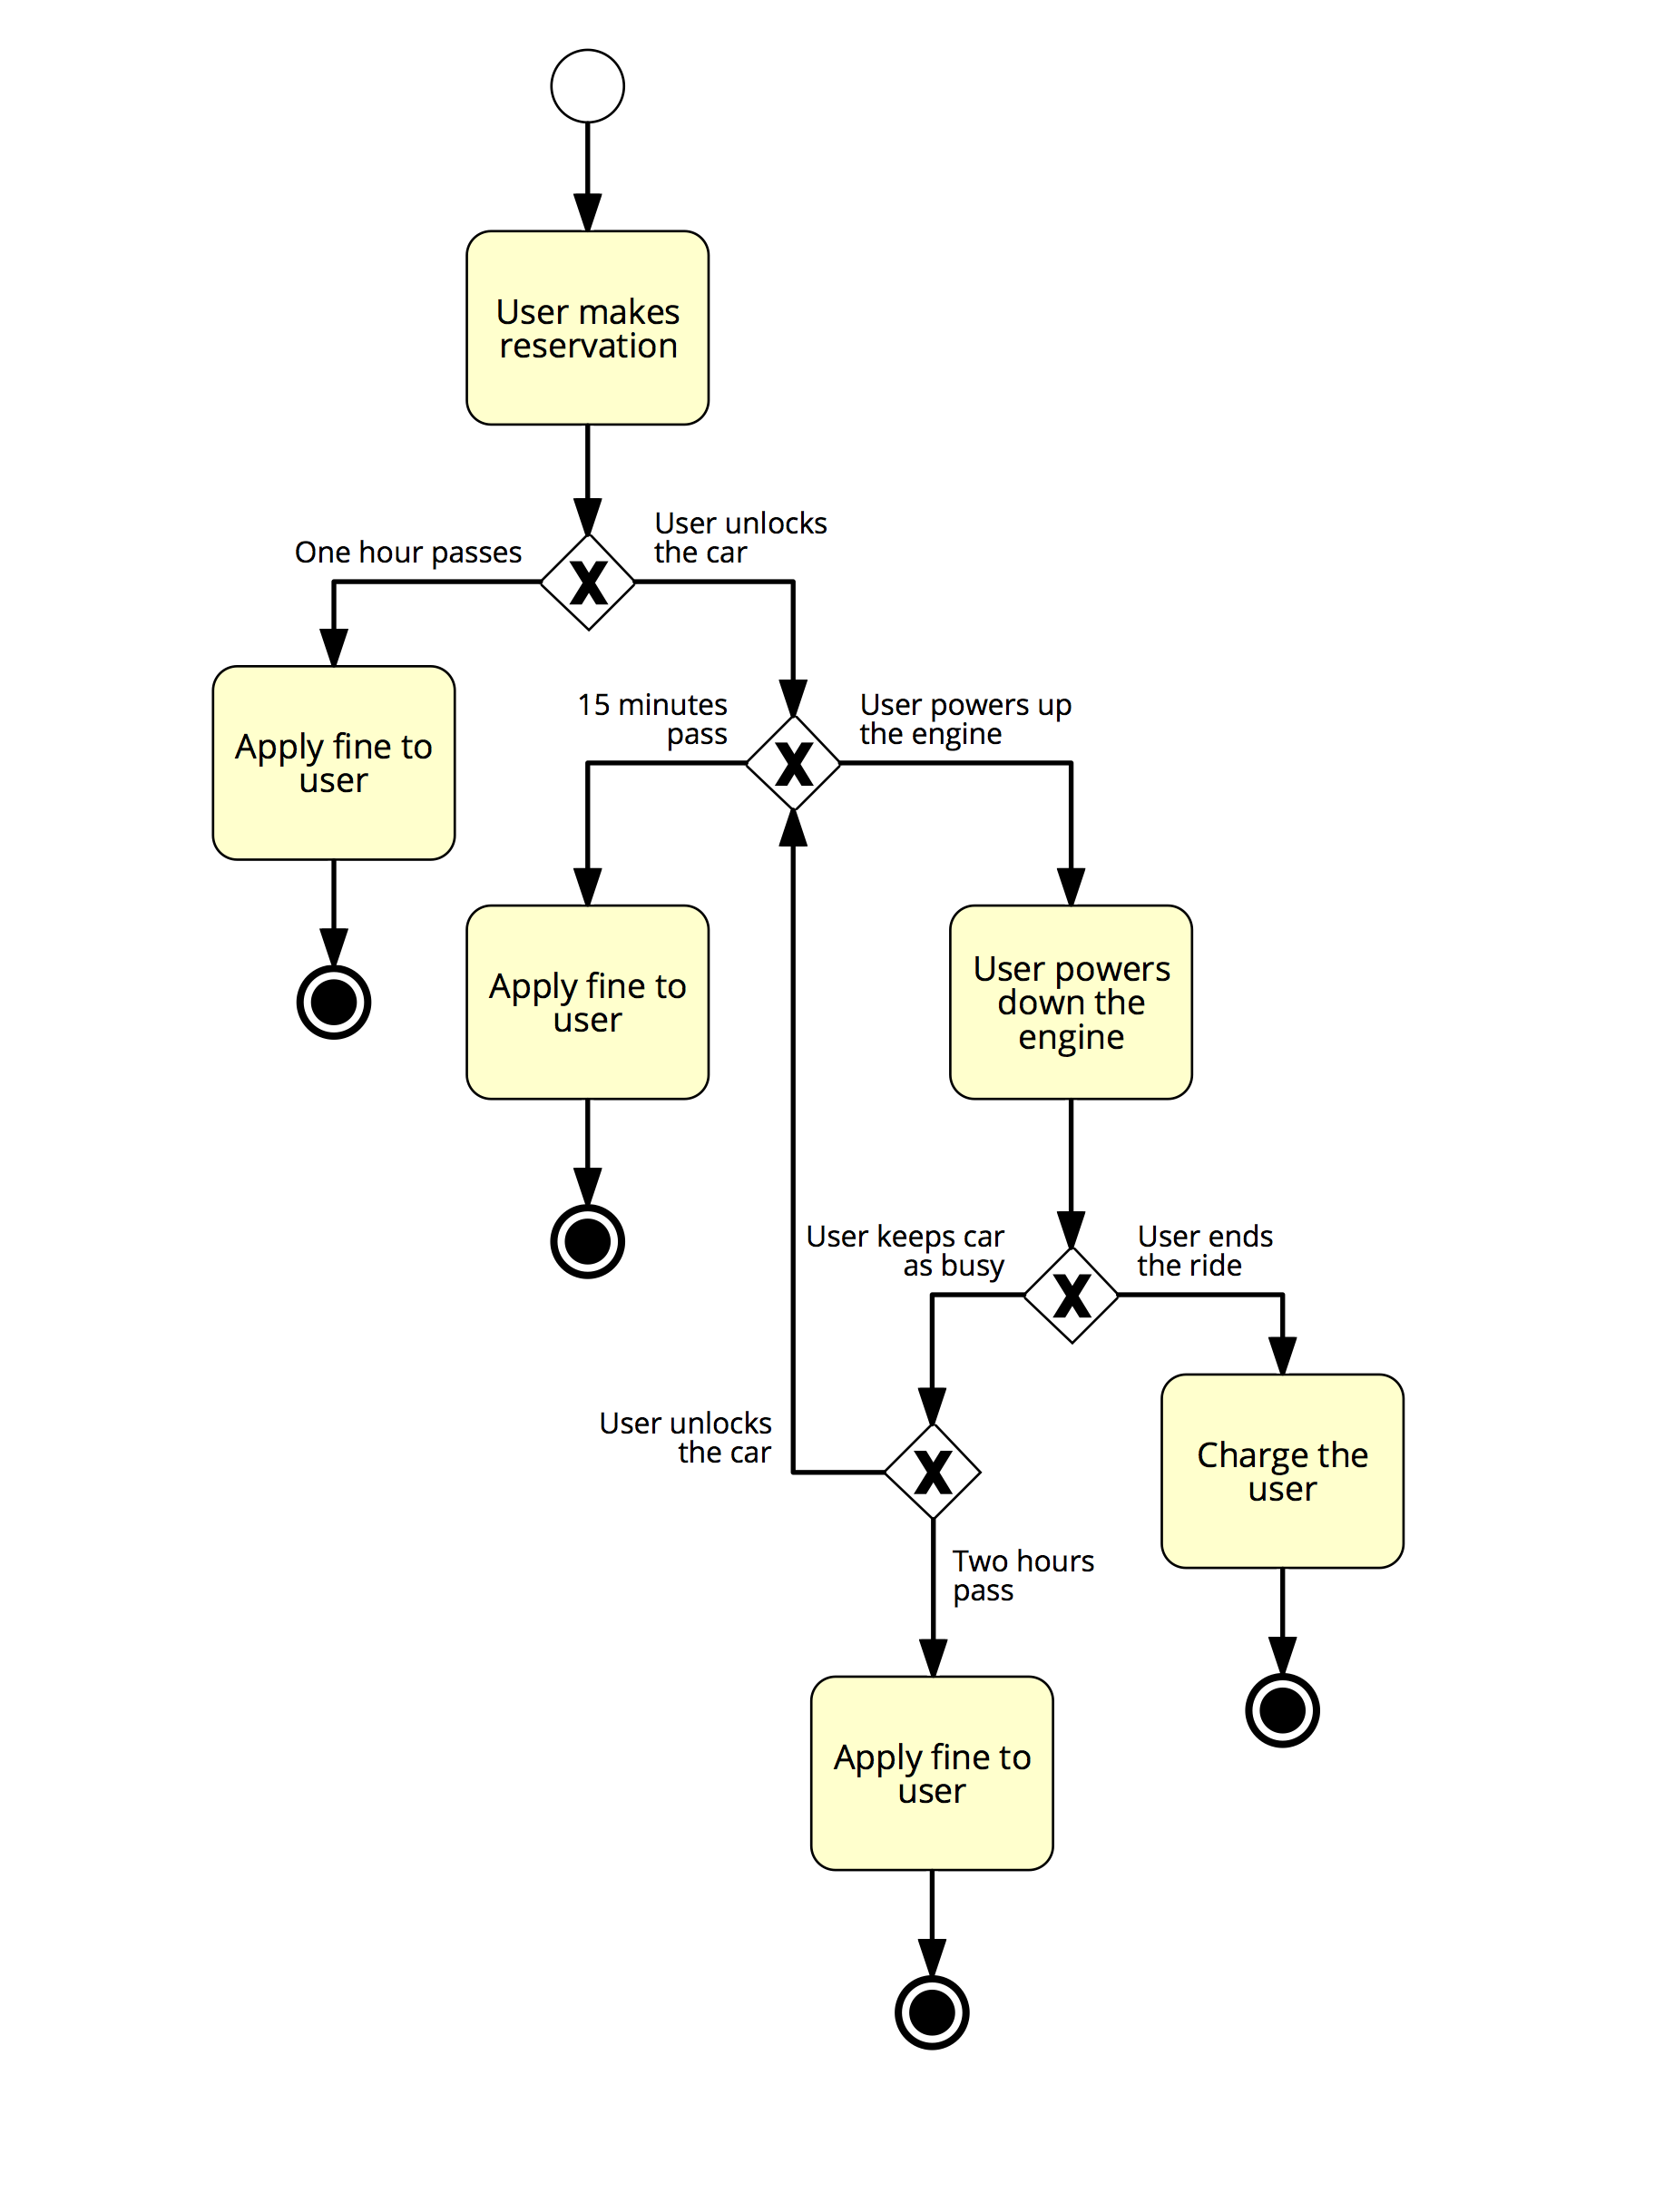
\includegraphics[width=6.25000in]{./FlowDiagrams/RideFlowAD.png}}

\newpage

\subparagraph{\texorpdfstring{Car State Diagram
\newline}{Car State Diagram }}\label{car-state-diagram}

\centerline{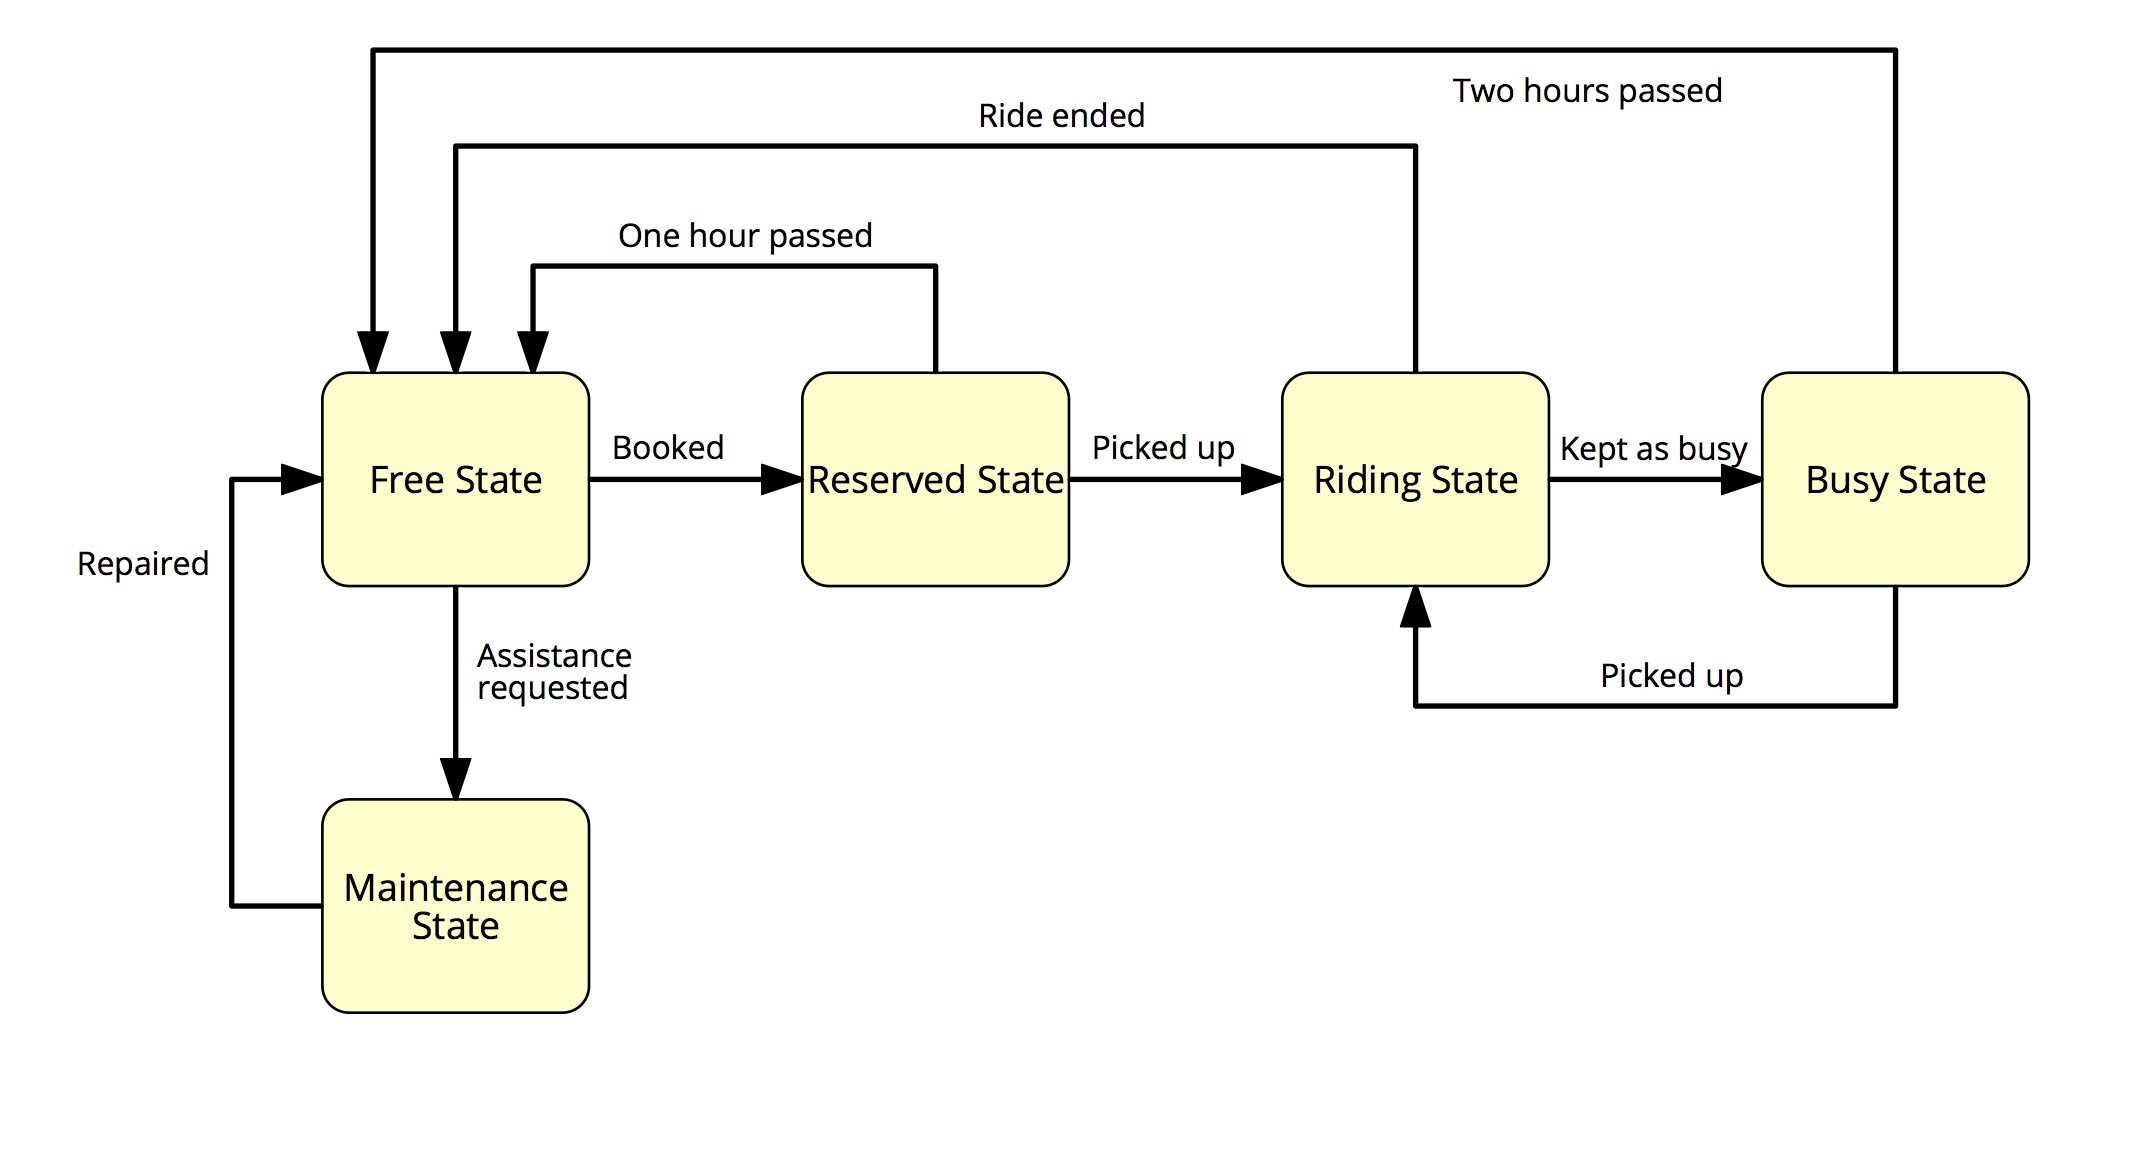
\includegraphics[width=6.25000in]{./FlowDiagrams/CarSD.png}}

\newpage

\subparagraph{\texorpdfstring{Discount/Penalty Activity Diagram
\newline}{Discount/Penalty Activity Diagram }}\label{discountpenalty-activity-diagram}

\centerline{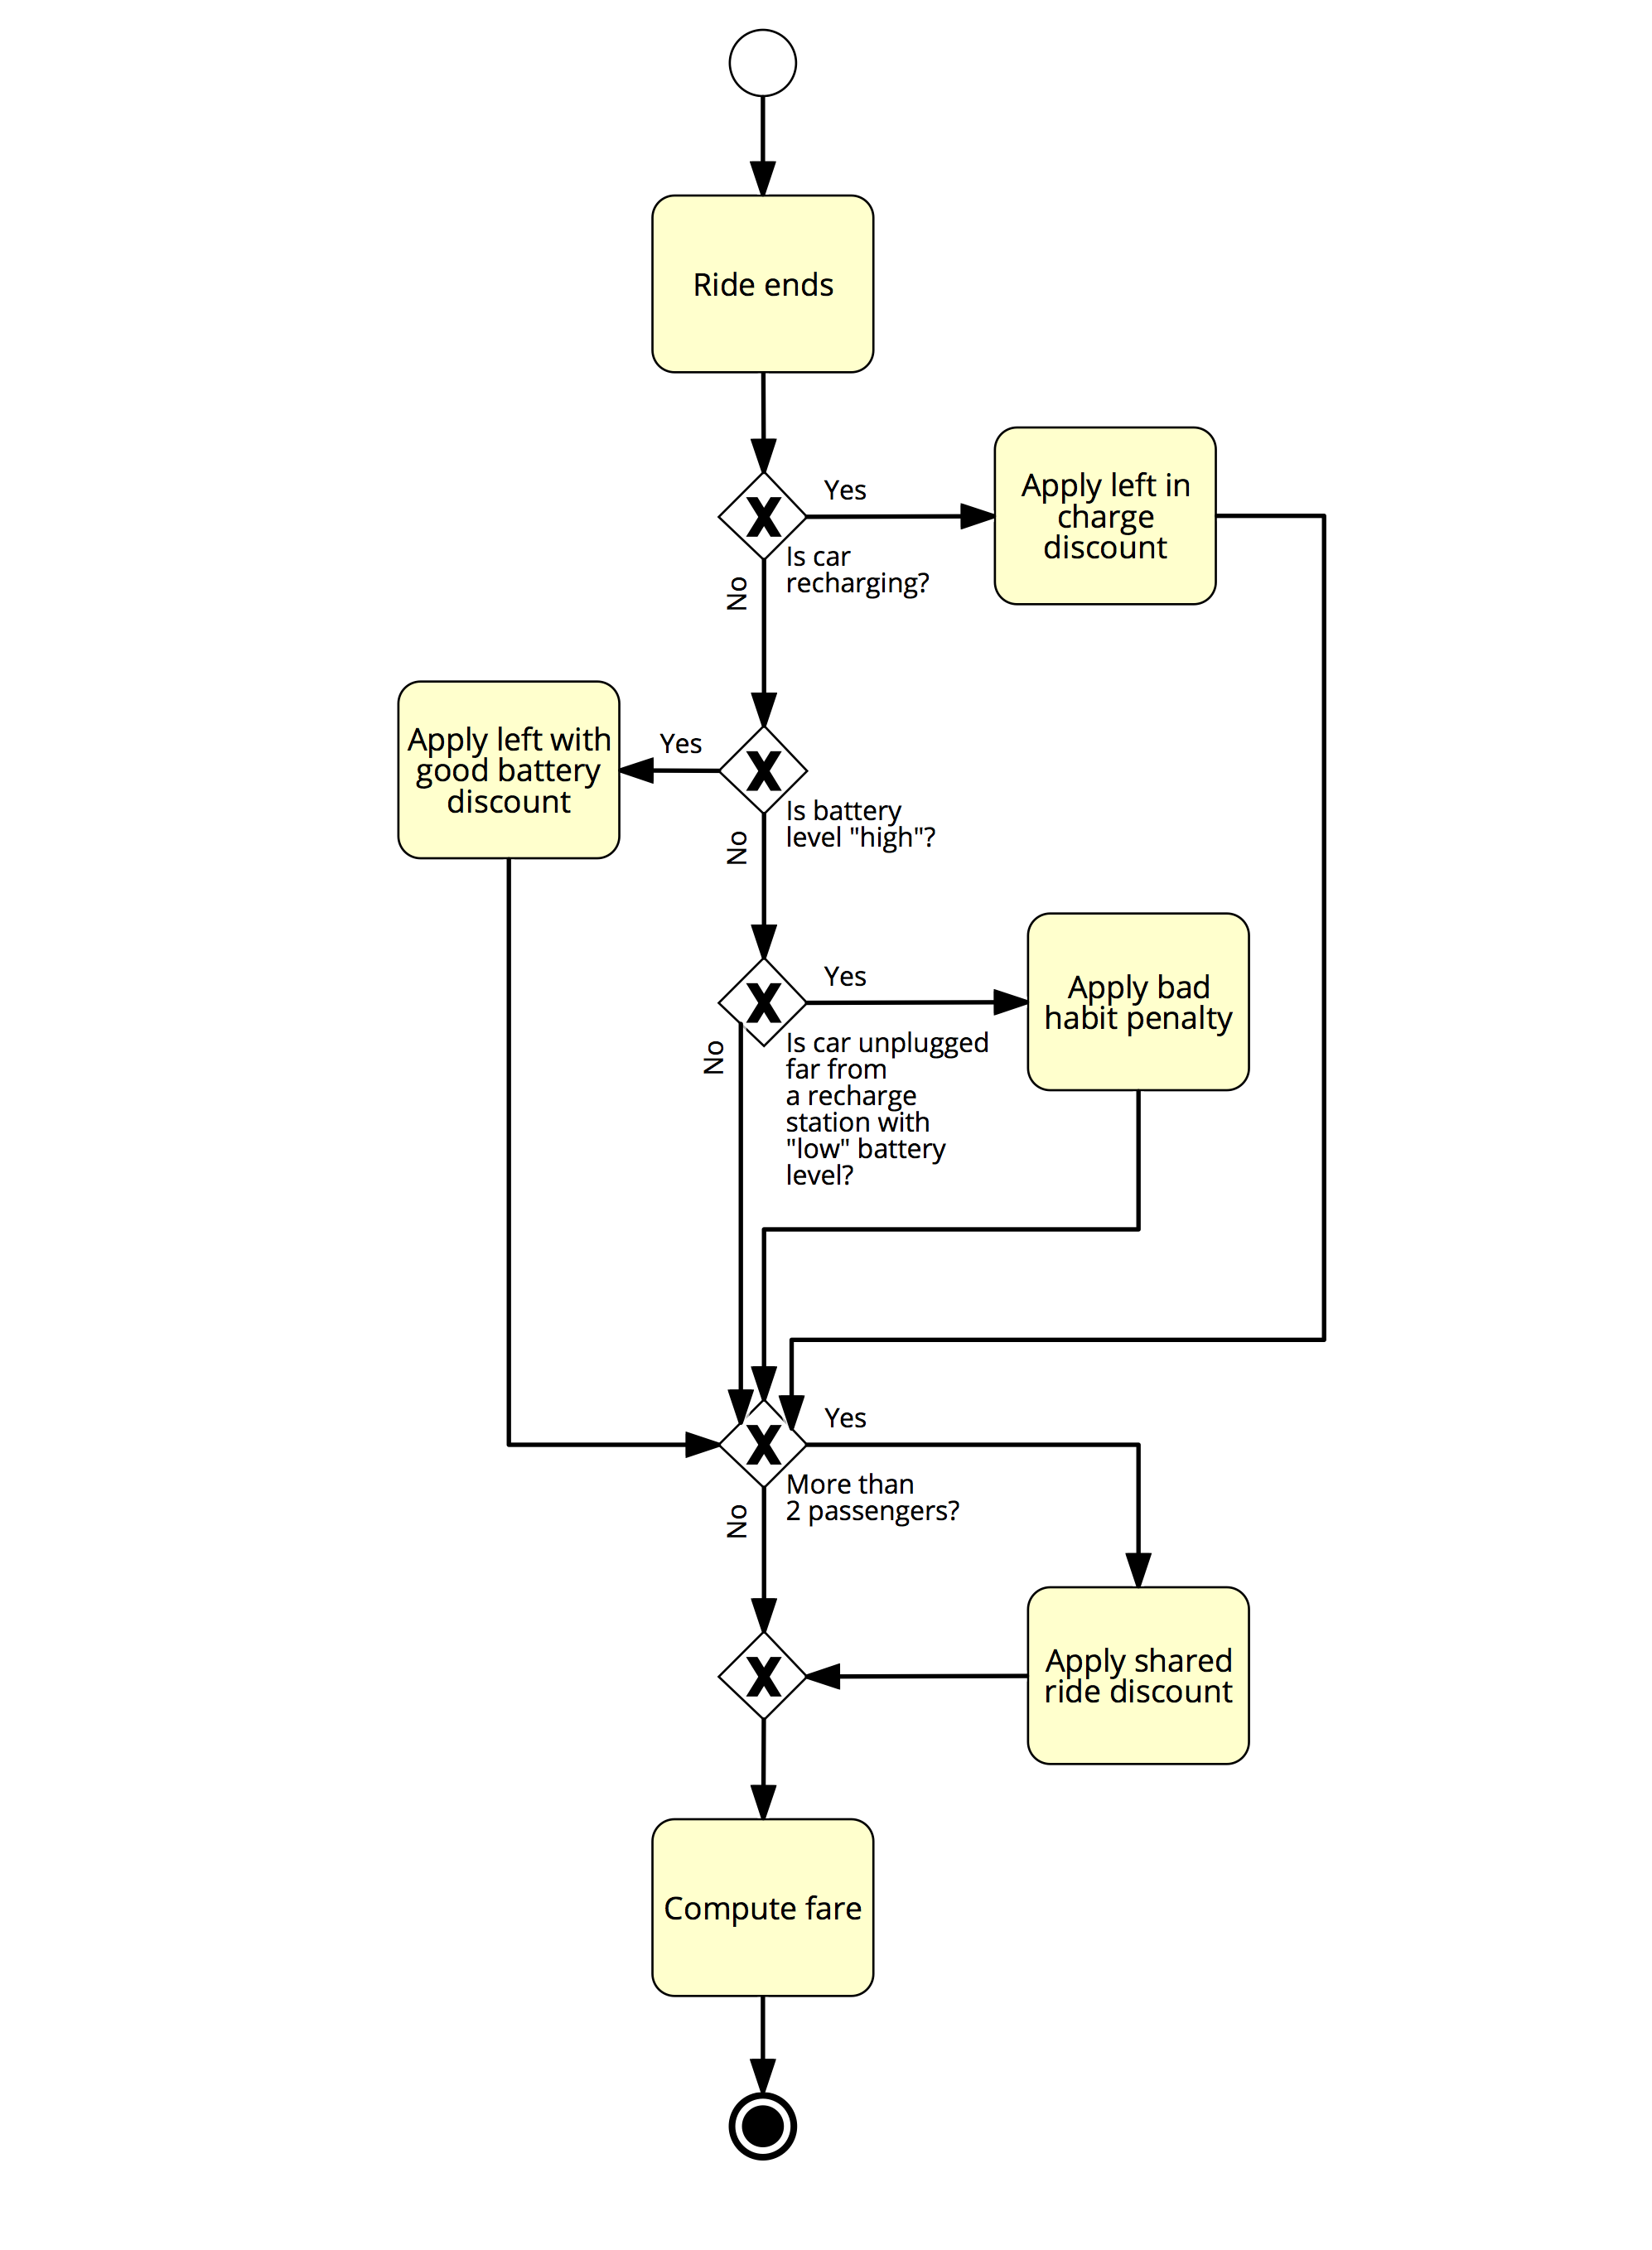
\includegraphics[width=6.25000in]{./FlowDiagrams/DiscountPenaltyAD.png}}

\newpage

\paragraph{Operator enrolls an assistance
request}\label{operator-enrolls-an-assistance-request}

\begin{longtable}[]{@{}ll@{}}
\toprule
\begin{minipage}[t]{0.29\columnwidth}\raggedright\strut
\textbf{Name}\strut
\end{minipage} & \begin{minipage}[t]{0.65\columnwidth}\raggedright\strut
Operator enrolls an assistance request\strut
\end{minipage}\tabularnewline
\begin{minipage}[t]{0.29\columnwidth}\raggedright\strut
\textbf{Goals}\strut
\end{minipage} & \begin{minipage}[t]{0.65\columnwidth}\raggedright\strut
G6\strut
\end{minipage}\tabularnewline
\begin{minipage}[t]{0.29\columnwidth}\raggedright\strut
\textbf{Actors}\strut
\end{minipage} & \begin{minipage}[t]{0.65\columnwidth}\raggedright\strut
Operator\strut
\end{minipage}\tabularnewline
\begin{minipage}[t]{0.29\columnwidth}\raggedright\strut
\textbf{Entry conditions}\strut
\end{minipage} & \begin{minipage}[t]{0.65\columnwidth}\raggedright\strut
The operator is logged into the system.\strut
\end{minipage}\tabularnewline
\begin{minipage}[t]{0.29\columnwidth}\raggedright\strut
\textbf{Flow of events}\strut
\end{minipage} & \begin{minipage}[t]{0.65\columnwidth}\raggedright\strut
\begin{itemize}
\tightlist
\item
  The operator enters the map screen.
\item
  The operator clicks on a new issue form the list.
\item
  The operator is redirected to a deep issue details screen.
\item
  The operator types in the form the details of the request.
\item
  The operator selects the facility of which the request must be sent
  to.
\item
  The operator hits the ``Send request'' button.
\item
  The system attaches the details of the car to the request and sends
  it.
\item
  The operator is redirected to the map screen.
\end{itemize}\strut
\end{minipage}\tabularnewline
\begin{minipage}[t]{0.29\columnwidth}\raggedright\strut
\textbf{Exit conditions}\strut
\end{minipage} & \begin{minipage}[t]{0.65\columnwidth}\raggedright\strut
The request is correctly enrolled to the specified facility. The
operator is back on the map screen.\strut
\end{minipage}\tabularnewline
\begin{minipage}[t]{0.29\columnwidth}\raggedright\strut
\textbf{Exceptions}\strut
\end{minipage} & \begin{minipage}[t]{0.65\columnwidth}\raggedright\strut
The request can't be enrolled or the operator forgot to fill in one of
the fields. In this case the system shows an error screen notifying the
problem and asking the operator to try again, then redirects him back to
the request screen.\strut
\end{minipage}\tabularnewline
\bottomrule
\end{longtable}

\newpage

\subparagraph{Assistance Request Sequence
Diagram}\label{assistance-request-sequence-diagram}

\centerline{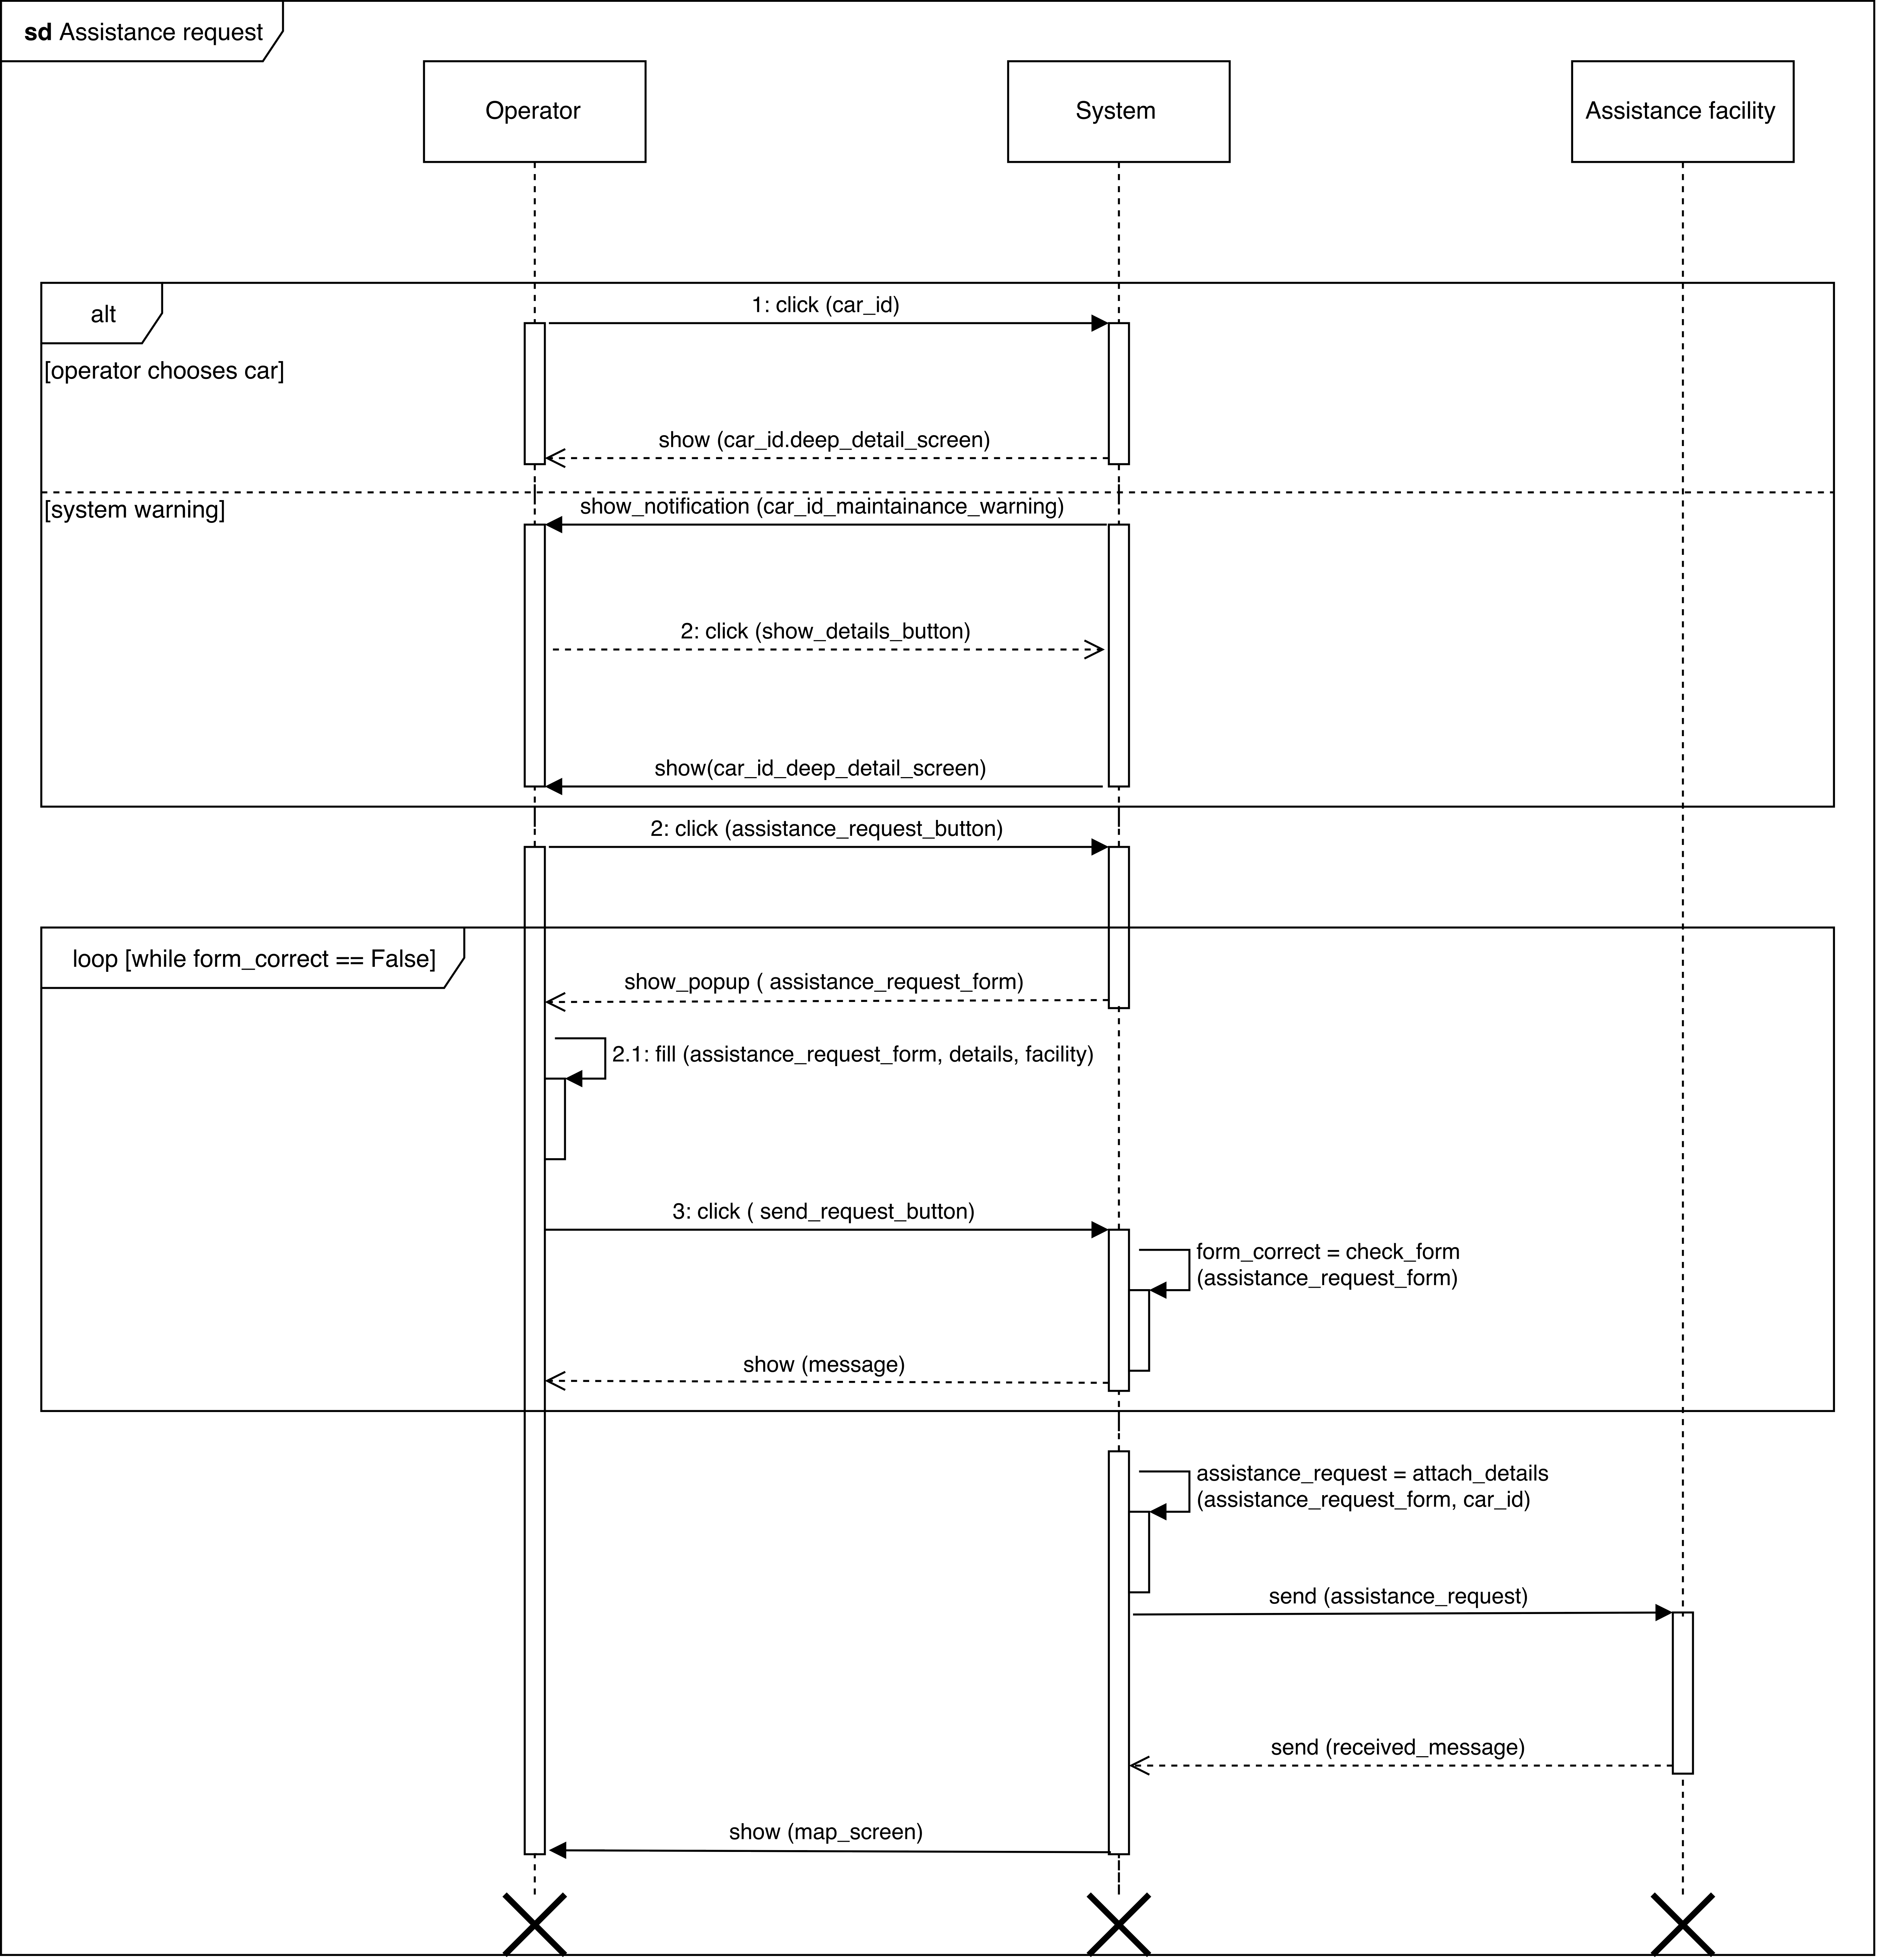
\includegraphics[width=6.25000in]{./FlowDiagrams/AssistanceRequestSD.png}}\newpage

\paragraph{Operator inserts a new safe
area}\label{operator-inserts-a-new-safe-area}

\begin{longtable}[]{@{}ll@{}}
\toprule
\begin{minipage}[t]{0.29\columnwidth}\raggedright\strut
\textbf{Name}\strut
\end{minipage} & \begin{minipage}[t]{0.65\columnwidth}\raggedright\strut
Operator inserts a new safe area\strut
\end{minipage}\tabularnewline
\begin{minipage}[t]{0.29\columnwidth}\raggedright\strut
\textbf{Goals}\strut
\end{minipage} & \begin{minipage}[t]{0.65\columnwidth}\raggedright\strut
G7\strut
\end{minipage}\tabularnewline
\begin{minipage}[t]{0.29\columnwidth}\raggedright\strut
\textbf{Actors}\strut
\end{minipage} & \begin{minipage}[t]{0.65\columnwidth}\raggedright\strut
Operator\strut
\end{minipage}\tabularnewline
\begin{minipage}[t]{0.29\columnwidth}\raggedright\strut
\textbf{Entry conditions}\strut
\end{minipage} & \begin{minipage}[t]{0.65\columnwidth}\raggedright\strut
The operator is logged into the system.\strut
\end{minipage}\tabularnewline
\begin{minipage}[t]{0.29\columnwidth}\raggedright\strut
\textbf{Flow of events}\strut
\end{minipage} & \begin{minipage}[t]{0.65\columnwidth}\raggedright\strut
\begin{itemize}
\tightlist
\item
  The operator enters the safe areas management screen.
\item
  The operator clicks on the ``New safe area'' button.
\item
  The operator is redirected to a map screen showing the set of safe
  areas.
\item
  The operator clicks on the polygonal drawing tool.
\item
  The operator is redirected on the vertices insertion screen.
\item
  The operator inserts the coordinates of the vertices clicking on the
  map.
\item
  The operator clicks the ``Confirm'' button.
\item
  The operator is redirected to the map screen now showing the new safe
  area.
\item
  The operator clicks on the ``Save and exit'' button.
\item
  The system generates the update details notification.
\item
  The system sends the update details notification to the users.
\item
  The operator is redirected to the initial terminal screen.
\end{itemize}\strut
\end{minipage}\tabularnewline
\begin{minipage}[t]{0.29\columnwidth}\raggedright\strut
\textbf{Exit conditions}\strut
\end{minipage} & \begin{minipage}[t]{0.65\columnwidth}\raggedright\strut
The new safe area is correctly inserted in the system and the update
details notification is successfully sent to the users. The operator is
redirected to the initial screen.\strut
\end{minipage}\tabularnewline
\begin{minipage}[t]{0.29\columnwidth}\raggedright\strut
\textbf{Exceptions}\strut
\end{minipage} & \begin{minipage}[t]{0.65\columnwidth}\raggedright\strut
\begin{itemize}
\tightlist
\item
  The operator has not defined a proper area (e.g.~not a valid shape).
  In this case the operator is redirected to the previous screen and
  notified of the mistake and must perform the action again correctly.
\end{itemize}\strut
\end{minipage}\tabularnewline
\bottomrule
\end{longtable}

\newpage

\subsection{11 Alloy Model}\label{alloy-model}

\lstinputlisting[language=alloy]{alloymodel.als}

\textbf{Result:} \newline
\centerline{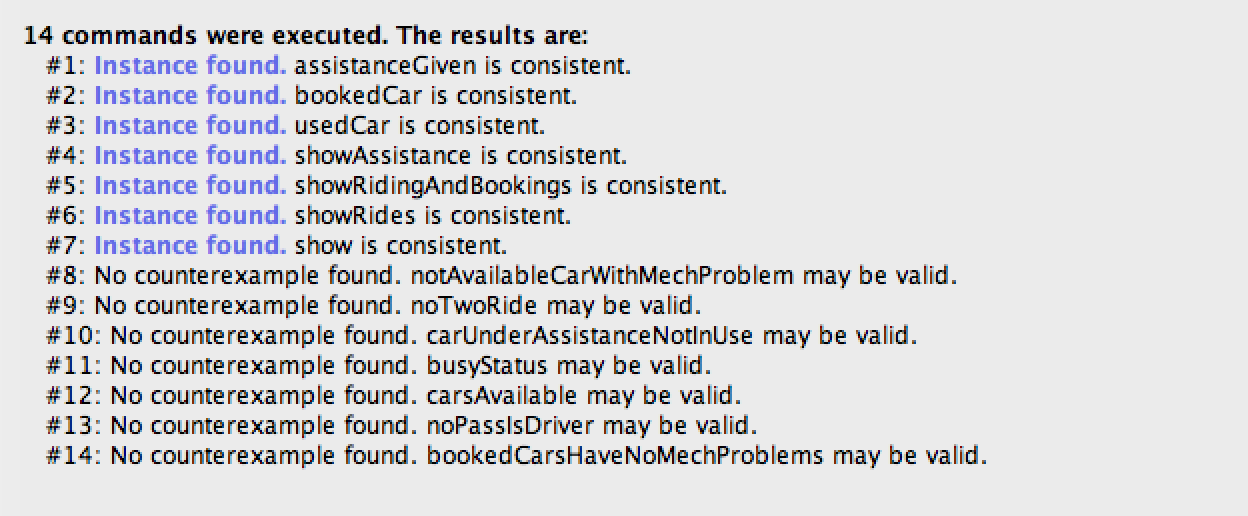
\includegraphics[width=1.00000\textwidth,height=1.00000\textwidth]{./alloyworlds/result.png}}
\newpage

\subsubsection{11.1 Generated Worlds}\label{generated-worlds}

\paragraph{Generic world}\label{generic-world}

Result of the show predicate: \newline
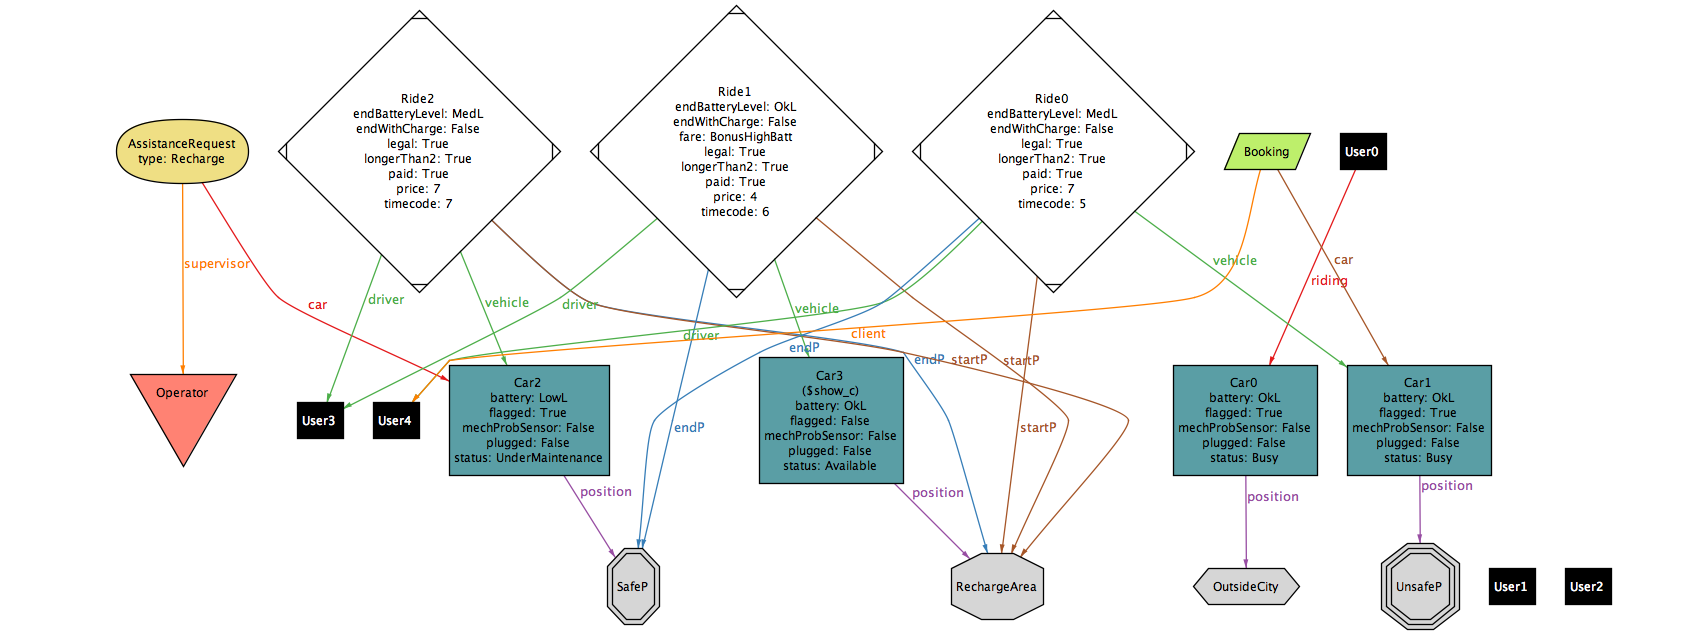
\includegraphics[width=1.00000\textwidth,height=1.00000\textwidth]{./alloyworlds/show.png}

\paragraph{Ride properties}\label{ride-properties}

Result of the showRides predicate: \newline
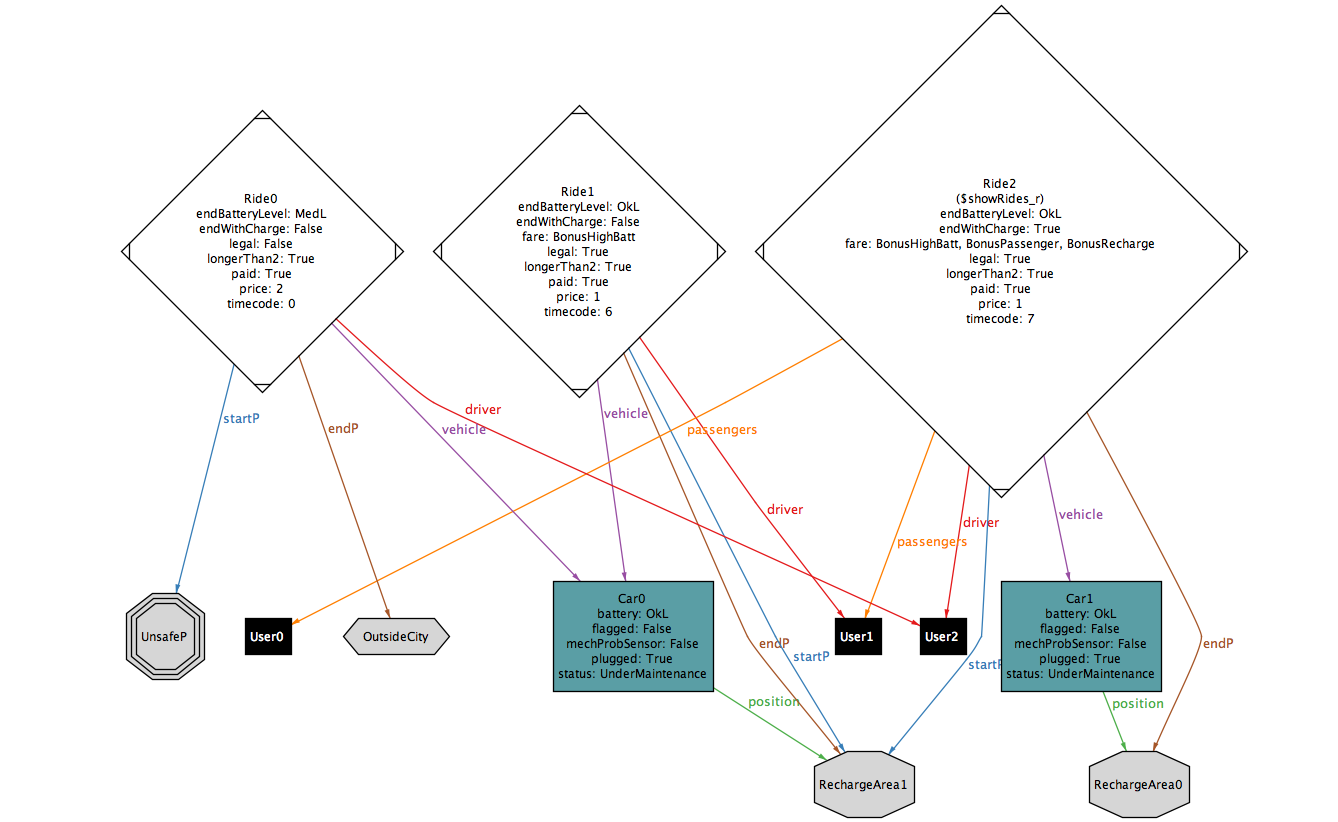
\includegraphics[width=1.00000\textwidth,height=1.00000\textwidth]{./alloyworlds/showRides.png}

\newpage

\paragraph{Booking and riding
properties}\label{booking-and-riding-properties}

Result of the showRidingAndBookings predicate:\newline \newline
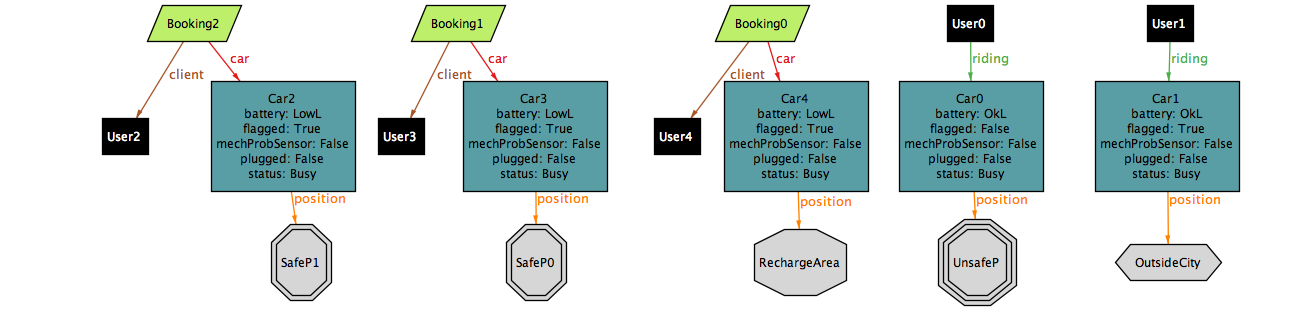
\includegraphics[width=1.00000\textwidth,height=1.00000\textwidth]{./alloyworlds/showRidingAndBookings.png}

\paragraph{Assistance properties}\label{assistance-properties}

Result of the showAssistance predicate:\newline
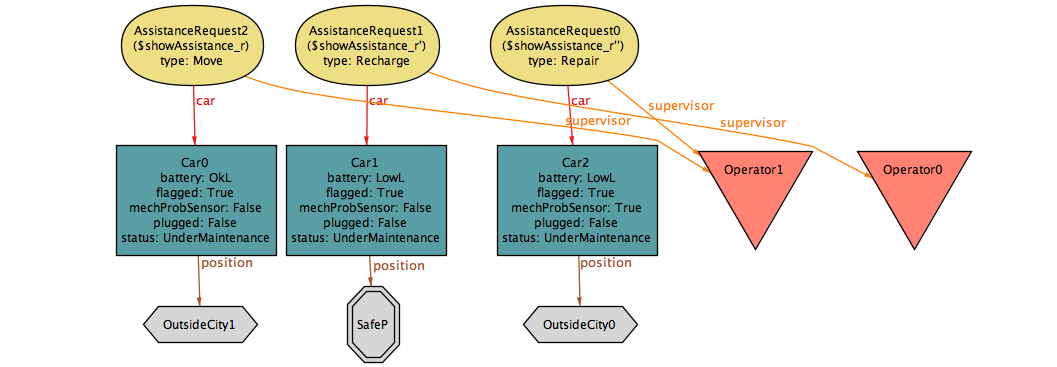
\includegraphics[width=1.00000\textwidth,height=1.00000\textwidth]{./alloyworlds/showAssistance.png}

\newpage

\paragraph{Dynamic Models}\label{dynamic-models}

Result of the usedCar predicate:\newline
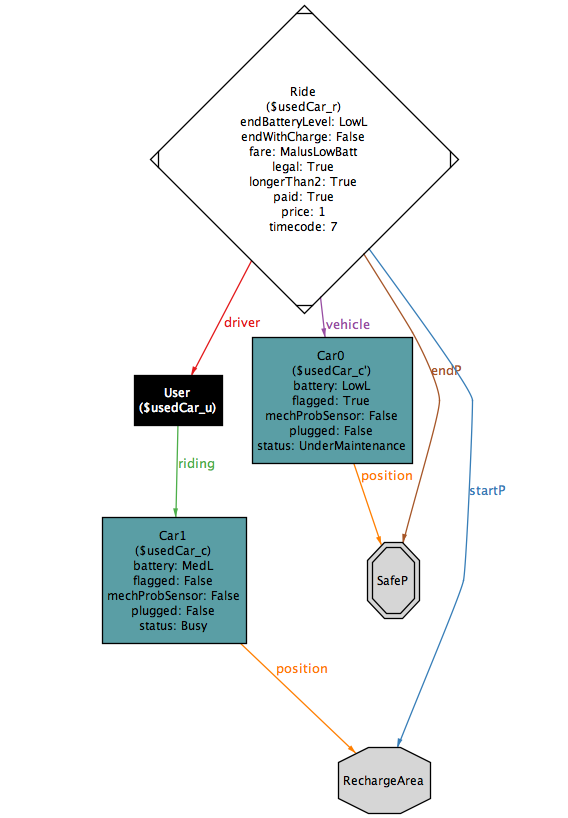
\includegraphics[width=1.00000\textwidth,height=1.00000\textwidth]{./alloyworlds/usedCar.png}

Result of the assistanceGiven predicate:\newline
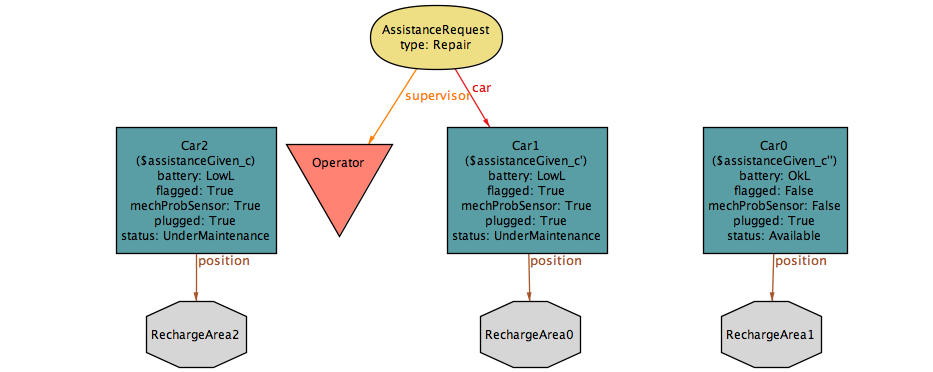
\includegraphics[width=1.00000\textwidth,height=1.00000\textwidth]{./alloyworlds/assistanceGiven.png}

\newpage

Result of the bookedCar predicate:\newline \newline
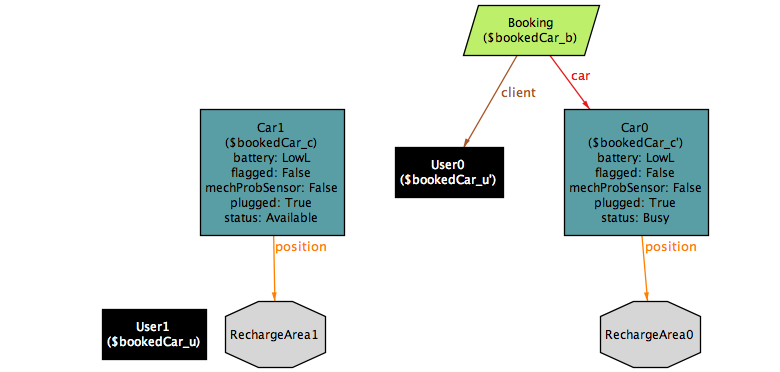
\includegraphics[width=1.00000\textwidth,height=1.00000\textwidth]{./alloyworlds/bookedCar.png}

\newpage

\subsection{12 Used tools}\label{used-tools}

\begin{itemize}
\tightlist
\item
  Atom (with MarkDown Preview Plus package) for writing Pandoc MarkDown
  with syntax highlighting and the preview feature.
\item
  Pandoc to craft the LaTeX document from the MD one and the pdf from
  the LaTeX.
\item
  TexShop to edit the LaTeX document(credits to
  \href{https://github.com/Angtrim/alloy-latex-highlighting}{\emph{Angtrim}}
  on GitHub for the Alloy syntax highlighting).
\item
  Alloy analyzer 4.2.
\item
  Signavio for the use case, class and activity diagrams.
\item
  Draw.io for the sequence diagrams.
\item
  Balsamiq for the GUI mockups.
\end{itemize}

\subsection{13 Reference material}\label{reference-material}

\begin{itemize}
\tightlist
\item
  Project assignment from : Assignments AA 2016-2017.pdf.
\item
  RASD example : RASD sample from Oct. 20 lecture.pdf.
\item
  IEEE standard on requirement engineering.
\end{itemize}

\subsection{14 Future Development}\label{future-development}

\begin{itemize}
\tightlist
\item
  Enhance the efficiency of the communications with the road operators.
\item
  Extend the customizability of the system (e.g.~the possibility to add
  more discounts/penalties).
\item
  Monitor the behaviour of the passengers, so that if they leave the
  ride earlier than the driver, the discount might not apply.
\end{itemize}

\subsection{15 Hours of work}\label{hours-of-work}

Each group member spent around 30 hours drafting the document. (The
commits on GitHub are not completely representative of the work done, a
good part of it has been done in group.)

\end{document}
